\documentclass{article}
\usepackage[utf8]{inputenc}
%\usepackage[T1]{fontenc}
\usepackage{natbib}
\usepackage{graphicx}
\usepackage{hyperref}
\usepackage[french]{babel}
\usepackage{url}
\usepackage[]{eurosym}
\usepackage{textcomp}

\usepackage{amsmath}

\usepackage{amssymb}

\usepackage{mathrsfs}

\usepackage[final]{pdfpages} 

%\title{ShareLaTeX project}
%\author{sylvain }
%\date{April 2017}



\renewcommand\contentsname{Table des matières}

 \setcounter{tocdepth}{2}


\begin{document}
\begin{titlepage}
	\centering
	
\includegraphics[scale=0.5]{./images/EIC.png}\\
	{\scshape\LARGE École Industrielle et Commerciale d'Andenne\par}
	\vspace{1cm}
	%{\scshape\Large Final year project\par}
	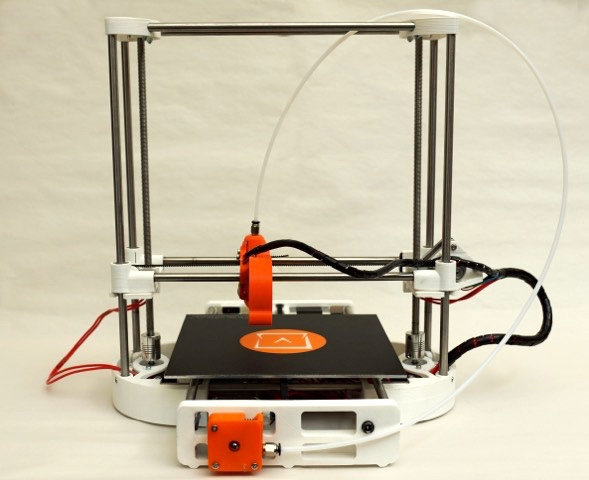
\includegraphics[scale=0.5]{./images/dagoma.png}
	\vspace{1.5cm}
	{\huge\bfseries Sensibilisation à l'Impression 3D \\ v2.0\par}
	\vspace{1,5cm}
	{\Large\itshape Sylvain DENIS\par}
	{\Large sept 2017\par}
\end{titlepage}



\newpage
\tableofcontents
\newpage

%    \part{Intitulé de la partie} (d'un usage assez rare pour un document de type article)
%    \section{Intitulé de la section}
%    \subsection{Intitulé de la sous-section}
%    \subsubsection{Intitulé de la sous-sous-section}


\part{Objectifs}
\begin{flushleft}
\textbf{\textit{Sensibilisation à l'impression 3D}}\hfill \break

L'étudiant sera capable :
\begin{itemize}
\item d'identifier les procédés d'impression et les technologies de fabrication numérique (fraisage, découpe laser, etc.)
\item de reconnaître les différents types d'imprimantes et les matériaux utilisés
\item de s'initier aux enjeux de propriété intellectuelle qui en découlent
\item de décrire le fonctionnement d'une imprimante 3D
\item d'appréhender les logiciels de dessin ou autres permettant des modélisations simples (identifier les différentes étapes depuis la création d'un objet jusqu'à son impression et associer les principales étapes du processus au logiciel adéquat)
\end{itemize}
\end{flushleft}

\begin{flushleft}
\textbf{\textit{Laboratoire de dessin assisté par ordinateur en trois dimensions}}\hfill \break

L'étudiant sera capable :\\
\textit{au départ d'un logiciel de modélisation préalablement installé sur une structure informatique opérationnelle ou tiré d'Internet,}
\begin{itemize}
\item d'exécuter l'application CAO telle que mise à disposition
\item de s'initier aux menus déroulants, aux commandes fondamentales, ... du logiciel
\item de différencier et de visualiser les différentes représentations d'un volume en mode filaire, surfacique et solide
\item de créer des volumes élémentaires en mode surfacique et en mode solide tels que : boîte, cône, coin, cylindre, sphère, tore,...
\item de déplacer, d'orienter et de positionner des volumes élémentaires dans l'espace
\item de visualiser un volume par ses arêtes cachées et par un ombrage ou un rendu
\item de modifier des fichiers d'un objet préconçu extraits d'un site Internet
\item de créer un fichier objet en vue de son impression (via des logiciels de conversion en GCODE)
\item de manipuler un logiciel de conversion en GCODE selon les options données (remplissage, épaisseur de couche, de coque,...)
\item d'imprimer un fichier GCODE
\end{itemize}
\end{flushleft}


\part{Théorie}
\section{Qu'est-ce que l'impression 3D ?}
\subsection{Petite Histoire de l'imprimante 3D}
\subsubsection{1952}
Kojima démontre les avantages de la fabrication par couches superposées.
\subsubsection{1967}
Swainson dépose un brevet aux États-Unis pour un système de durcissement de résine par double rayon lumineux.
\subsubsection{1972 - Hergé nous en parle}
\begin{figure}[h!]
\centering
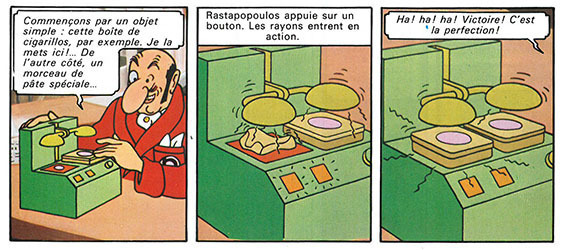
\includegraphics[scale=0.6]{./images/tintin.png}
\end{figure}
C'est dans Tintin et le Lac aux Requins, de Hergé, qu'est avancée pour la toute première fois l'idée d'une machine capable de reproduire un objet en trois dimensions à partir d'une copie originale, par le professeur Tournesol.
\subsubsection{1981}
Kodama publie trois méthodes de solidification holographique.
\subsubsection{1982}
Chuck Hull mène des recherches sur la stéréolithographie.
\begin{figure}[h!]
\centering
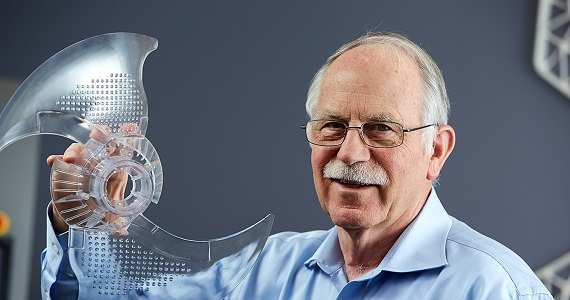
\includegraphics[scale=0.3]{./images/charleshull.jpg}
\end{figure}
\subsubsection{1984}
Charles Hull dépose le brevet 4575330 d’utilisation de la stéréolithographie.
\subsubsection{1986 - Commercialisation de la première machine}
Création de 3D Systems. D’autres acteurs entrent en jeu.

Officiellement commercialisée en 1986, cette machine reposait sur le principe de Stéréolytographie.
On ne parle pas encore d'impression 3D et la machine est une espèce de prototype testé par de rares entreprises triées sur le volet.

Cette première imprimante 3D débouchera sur le premier modèle de série en 1988 : la SLA-2502 de 3D Systems.
L'imprimante sert, alors, aux industriels à créer des objets pour tester leur design avant de décider la production des pièces en série.

\begin{figure}[h!]
\centering
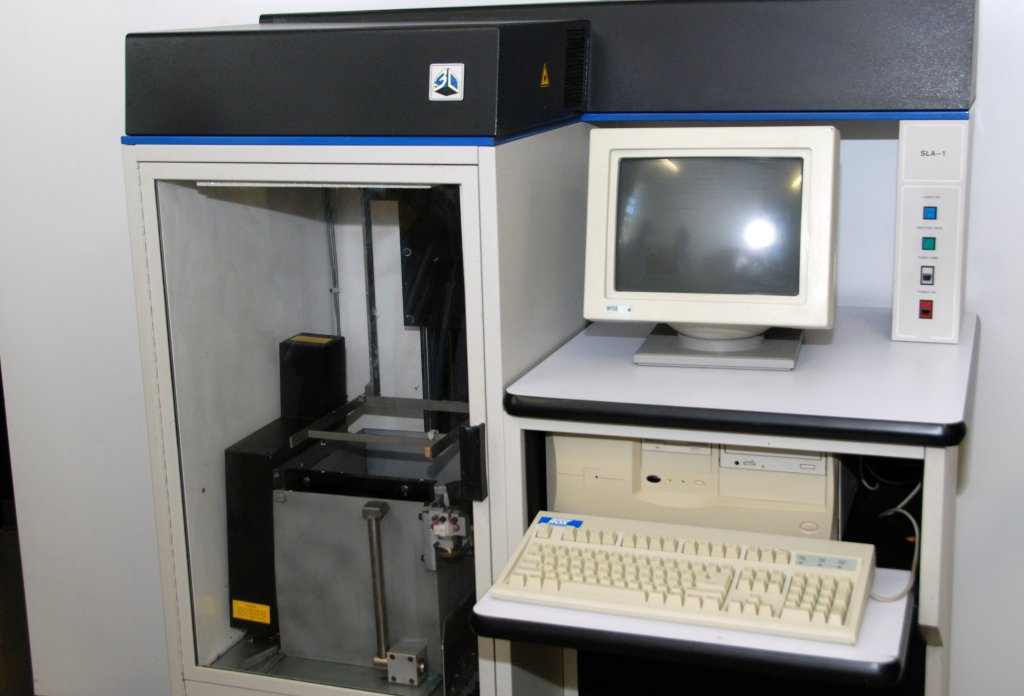
\includegraphics[scale=0.3]{./images/SLA-2502-3D-Systems.png}
\end{figure}
\subsubsection{1987}
Le prototypage rapide devient une réalité commerciale.
\subsubsection{1989}
Lancement de Stratasys et des premières imprimantes FDM.
\subsubsection{1990}
La fabrication additive est utilisée pour la réalisation de moules.
\subsubsection{1990-1992 - L'impression couche après couche}
Ce n'est pas encore parfait loin de là mais le potentiel énorme de l'impression 3D se dévoile avec la création couche après couche d'objets 3D.

Un rayon UV tape dans un espèce de liquide visqueux. Pas super pratique mais plutôt efficace; l'impression 3D prouve qu'elle est capable de créer des pièces complexes. C'est toujours le procédé de Stéréolytographie qui fait ses preuves.
\subsubsection{1995}
Z Corporation lance les premières imprimantes 3DP.
\subsubsection{1996}
Premières mentions des machines industrielles comme « imprimantes 3D ».
\subsubsection{1999 - La première prothèse implantée sur un être humain.}
Les chercheurs et les ingénieurs créent une espèce de prothèse permettant d'accompagner l'agrandissement de la vessie d'un patient. Outre la contrainte de devoir créer un « objet » adapté à la physionomie du malade, il convient de trouver un système réduisant les risques de rejets. La pièce est donc enrobée de cellules du patient. Cette étape constitue une avancée majeure en ouvrant de nouvelles perspectives à la médecine.
\subsubsection{2000}
La fabrication additive est utilisée pour des pièces de production.
\subsubsection{2002 - Un premier rein fonctionnel}
C'est encore la même équipe de scientifique qui est à la base de cette prouesse (bio) médicale. Cette fois les universitaires du laboratoire Wake Forest Institute for Regenerative Medicine recréent un rein fonctionnel. Capable de filtrer le sang et de diluer l'urine, il est greffé sur des animaux et ouvre la voie à la création d'organes et de tissus à des buts médicaux.

Vidéo vers TED avec traduction en francais :

http://www.ted.com/talks/anthony\_atala\_printing\_a\_human\_kidney

\subsubsection{2005 - Lancement du RepRap Project}
2005 est une date clé. Le Dr Adrian Boyier et son équipe de l'Université de Bath imaginent une prouesse technologique en lançant la construction d'une imprimante 3D capable de créer les pièces utiles à son fonctionnement. 

Leur but ?

Rendre le plus accessible possible l'impression 3D où une machine auto-replicante « viraliserait » son usage et les services qu'elle peut apporter.
\begin{figure}[h!]
\centering
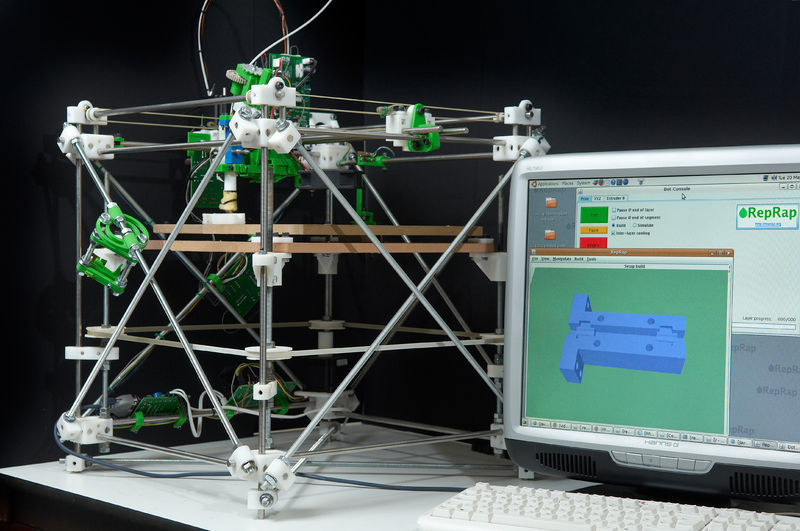
\includegraphics[scale=0.25]{./images/Darwin.png}
\end{figure}
\subsubsection{2007-2008 - Le RepRap Project abouti | Shapeways.com ouvre}
Le project RepRap réussi son pari. Leur première imprimante auto-réplicante sort. Darwin permet à un possesseur de créer d'autres machines pour son réseau proche.
C'est cette année là que sort la version Beta de la boutique de plans en ligne Shapeways.com.
Designers, architectes et ingénieurs peuvent créer des plans de manière conjointe et faire imprimer des objets complexes à prix abordable.
\subsubsection{2009 - MakerBot Industries à l'assaut du grand public}
Cette année là, la société MakerBot Industries propose à la vente un Kit DIY (Do It Yourself) à l'attention des particuliers. Tout le monde peut désormais posséder chez soi une imprimante 3D fonctionnelle à prix abordable.
\begin{figure}[h!]
\centering
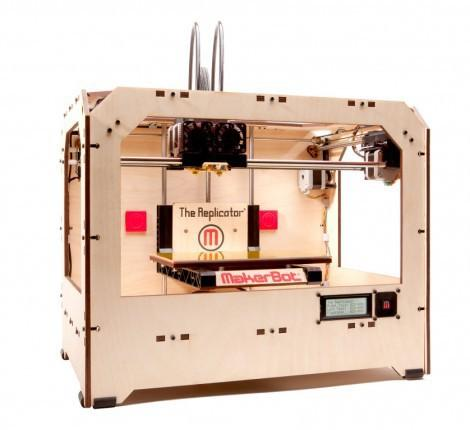
\includegraphics[scale=0.35]{./images/the-replicator.jpg}
\end{figure}
\newpage
\subsubsection{2010 - Un vaisseau sanguin imprimé avec une imprimante spéciale}
L'impression 3D à vocation médicale fait son petit bout de chemin mais, à la fin 2010, tout s'accélère. En décembre 2010, une équipe de chercheur parvient à créer avec une bio-imprimante 3D Organovo, un vaisseau sanguin fonctionnel.
\subsubsection{2011 - Un premier drone à 5000 Livres Sterling (+/-6500 \euro)}
Les ingénieurs de l'Université de Southampton parviennent à créer un avion sans pilote en une semaine pour le prix de 5000 Livres Sterling. Sulsa (c'est le nom de cet avion) mesure prêt de 2m d'envergure et est propulsé par un moteur électrique lui permettant d'atteindre la vitesse de 160km/h.\\
Imprimées grâce à la technologie SLS, les pièces du fuselage ont été produites en un temps record et avec une finesse remarquable.
\begin{figure}[h!]
\centering
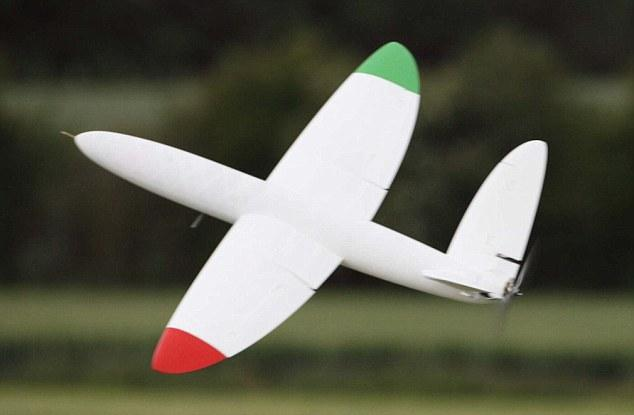
\includegraphics[scale=0.4]{./images/sulsa.jpg}
\end{figure}
\subsubsection{2011 - Après l'avion : la voiture}
Lors de la conférence TedX de Winnipeg au Canada, la société Kor Ecologic présente Urbee, une voiture dont la carosserie est complètement composée de pièces imprimées à l'aide d'une imprimante 3D. Urbee est « eco-friendly » et est dessinée pour consommer le moins de carburant possible. 1,18 litres au cent kilomètre sur autoroute et moitié moins en ville. On estime qu'elle coûterait entre 10000 et 50000 dollars si le projet commercial est viable.
\begin{figure}[h!]
\centering
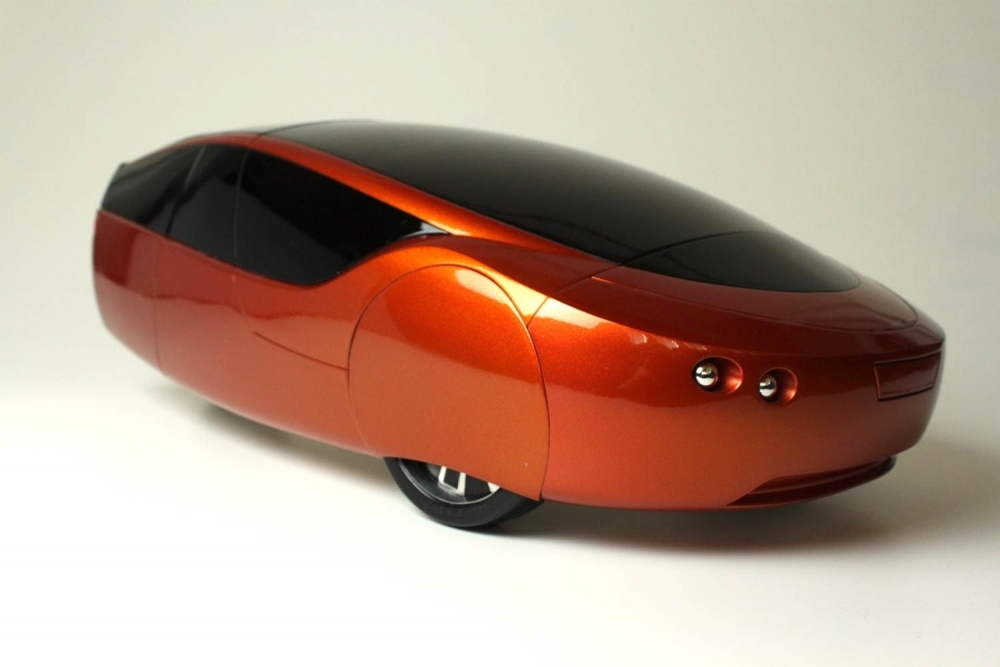
\includegraphics[scale=0.3]{./images/urbee.jpg}
\end{figure}
\subsubsection{2011 - L'or et l'argent en impression Grand Public}
i.materialise.com propose l'impression d'objets en or ou en argent. Plus que jamais le monde de l'imprimante 3D fait les yeux doux aux artisans, bijoutiers et « breloquiers » indépendants. Plus besoin de moules pour tirer des pièces en série, le bijou est unique et à prix réduit.
\subsubsection{2012 - Une prothèse de maxillaire inférieur posée sur une octogénaire}
C'est l'aboutissement du travail d'une équipe de chercheurs et d'ingénieurs Néerlandais : une prothèse de maxillaire posées sur une femme de 83 ans qui souffrait d'une infection à la mâchoire. Bien entendu, la prothèse est parfaitement ajustée à son hôte mais elle vise principalement à étudier la reconstruction des tissus osseux.
\subsubsection{2013 - Un arme à feu fonctionnelle}
Triste jour pour l'impression 3D avec l'un de ses plus gros buzz : la diffusion d'une vidéo, puis plus conséquemment, des plans d'une arme à feu. Le tout fait polémique et remonte jusqu'au gouvernement américain qui interdit leurs diffusions. Sauf que quand cela arrive, les plans ont déjà été téléchargés 100 000 fois.
\begin{figure}[h!]
\centering
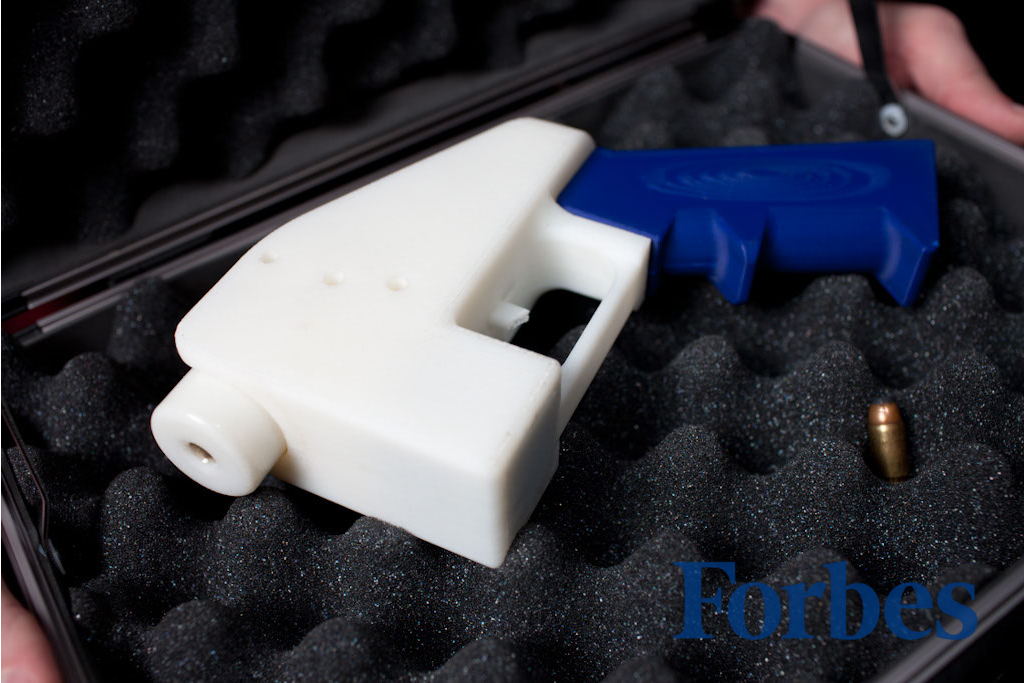
\includegraphics[scale=0.3]{./images/liberator.png}
\end{figure}
\subsubsection{2014 - Un plâtre révolutionnaire "imprimé" en 3D}
Jake Evill est diplômé de l'université Victoria de Wellington (Nouvelle-Zélande) et a inventé un tout nouveau genre de dispositif pour permettre aux os cassés de nos membres de se réparer sans tous les inconvénients liés aux éternels plâtres. Ce prototype est plus souple qu'un plâtre rigide et permet donc une meilleure mobilité. De plus, le plâtre est suffisamment solide sur la partie où l'os est fracturé, afin de mieux le protéger et d'éviter qu'il ne bouge, et est entièrement recyclable et imperméable à l'eau. 
\newpage
\subsection{Comment ça marche ?}
L'impression 3D n'est pas une technologie qui fonctionne d'une seule et même manière. Il existe, en effet, une multitude de procédés permettant d'imprimer un objet en 3D. Si les techniques d'impression sont différentes sur la forme, le principe reste toujours le même. Il consiste à superposer des couches de matières avec une imprimante 3D selon les cordonnées transmises par un fichier 3D.
\subsubsection{Fonctionnement d"une imprimante 3D}
L'impression 3D fonctionne selon plusieurs procédés, qui diffèrent selon le type d'imprimante 3D utilisée. On peut classer ces procédés dans trois grands groupes :
\begin{itemize}
\item Le dépôt de matière
\item La solidification par la lumière
\item L'agglomération par collage
\end{itemize} \hfill

Ces trois procédés fonctionnent selon le même principe de base, c'est à dire superposer des couches de matières selon les coordonnées d'un fichier 3D. La différence se situe sur la manière dont sont déposées et traitées ses couches, ainsi que le type de matériau utilisé.\hfill
\newline
Pour la plupart des procédés employés, l'utilisateur a besoin :
\begin{itemize}
\item d'une imprimante 3D
\item de consommable (filament, poudre...)
\item d'un fichier 3D (au format STL ou OBJ)
\item d'un logiciel de slicing pour trancher le fichier et transmettre les indications à l'imprimante
\item d'un ordinateur (ou assimilé)
\end{itemize}\hfill \break
La manière d'exporter les fichiers vers l'imprimante diffère selon les marques et les modèles :
\begin{itemize}
\item câble USB
\item Wi-Fi
\item carte SD
\end{itemize}

\subsubsection{L'impression par dépôt de matière}
\paragraph{FDM ou FFF} \hfill

La majorité des imprimantes 3D personnelles fonctionnent selon ce principe. FDM est l'acronyme anglais de Fused Deposition Modeling qui signifie modelage par dépôt de filament en fusion. Ce procédé qui a été inventé en 1988 par la société Stratasys, est une marque déposée. On parle aussi de FFF (Fused Filament Fabrication) voir même de MPD (Molten Polymer Deposition) qui sont eux des termes libres de droits. Cette technique consiste à déposer couche par couche un filament de matière thermoplastique fondu à 200\degres C (en moyenne) qui en se surperposant donne forme à l'objet. La tête d'impression se déplace selon les coordonnées X, Y et Z (longueur, largeur et hauteur) transmises par un fichier 3D correspondant au modèle 3D de l'objet à imprimer. Limitée pendant longtemps à des matériaux de type plastique tels que les classiques PLA et l'ABS, l'impression 3D voit arriver de nouveaux filaments composites à base de métal (cuivre, bronze...) et même de bois. Plus rarement certaines machines utilisent des cires ou des polycarbonates. Aujourd'hui l'industrie agroalimentaire et la médecine s'emparent peu à peu de cette technique pour imprimer des aliments et des cellules en adaptant la tête d'extrusion.
\begin{figure}[h!]
\centering
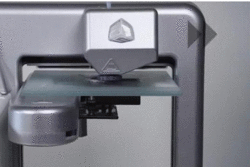
\includegraphics[scale=0.8]{./images/fdm.png}
\end{figure}
\begin{figure}[h!]
\centering
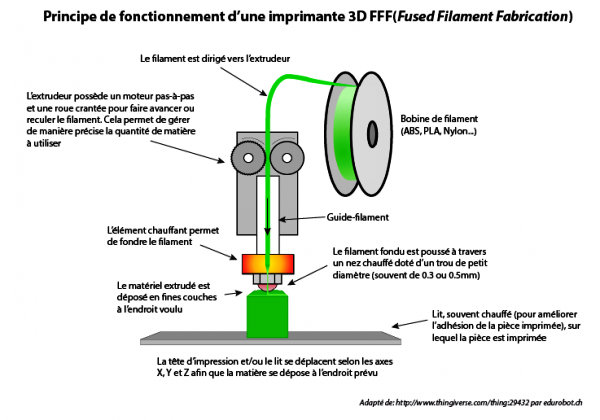
\includegraphics[scale=0.55]{./images/fonctionnement-imprimante-3d.png}
\end{figure}
\newpage
\subsubsection{Solidification par la lumière}
\paragraph{Stéréolithographie ou SLA} \hfill

La stéréolitographie est la première technique d'impression 3D à avoir été mise en évidence.
Si la paternité de ce procédé est souvent attribuée à l'américain Charles Hull fondateur de 3D Systems, on doit en fait cette invention à trois français (Alain le Méhauté, Olivier de Witte et Jean Claude André) dont leurs brevets bien que déposés 3 semaines plus tôt (16 juillet 1984), n'ont malheureusement pas été renouvelés. \hfill

Appelée aussi SLA (Stéréolithographie Apparatus), cette technique consiste à solidifier un liquide photosensible par le biais d'un rayon laser ultraviolet.

Les imprimantes fonctionnant par SLA ont quatre parties principales:
\begin{itemize}
\item un réservoir qui peut être rempli avec un liquide photopolymère
\item une plate-forme perforée qui est descendue dans le réservoir
\item un rayonnement ultraviolet (UV)
\item un ordinateur commandant la plate-forme et le laser
\end{itemize}\hfil

Tout comme la FDM, l'imprimante va dans un premier analyser le fichier CAO, puis en fonction de la forme de l'objet va lui ajouter des fixations temporaires pour maintenir certaines parties qui pourraient s'affaisser. Le laser va, ensuite, commencer par toucher et durcir instantanément la première couche de l'objet à imprimer. Une fois que la couche initiale de l'objet a durci, la plate-forme est abaissée, est ensuite exposée une nouvelle couche de surface de polymère liquide. Le laser trace à nouveau une section transversale de l'objet qui colle instantanément à la pièce durcie du dessous.\hfill

Ce processus se répète encore et encore jusqu'à ce que la totalité de l'objet ce soit formé et soit entièrement immergé dans le réservoir. La plateforme va ensuite se relever pour faire apparaître l'objet fini en trois dimensions. Après qu'il ai été rincé avec un solvant liquide pour le débarrasser de l'excès de résine, l'objet est cuit dans un four à ultraviolet pour durcir la matière plastique supplémentaire.\hfill

Les objets fabriqués selon la stéréolithographie ont généralement une bonne qualité de finition et de détail (0,0005 mm), on obtient des surfaces bien lisses et régulières. Qualitativement, elle fait partie des meilleurs techniques d'impression 3D actuellement. La durée nécessaire pour créer un objet avec cette technique dépend également de la taille de la machine utilisée. La SLA a aussi l'avantage de pouvoir produire de grosses pièces (de plusieurs mètres). Pour ces objets là, il faudra plusieurs jours, quelques heures pour les plus petites.\hfill

Parmi ces inconvénients, un coût plus élevé que la FDM et un panel de matériaux et des coloris plus limité du fait des polymères utilisés comme matière première. Les solvants et les liquides polymères dégageant par ailleurs des vapeurs toxiques durant l'impression, votre local devra être équipé d'une hotte aspirante pour l'aération.
\begin{figure}[h!]
\centering
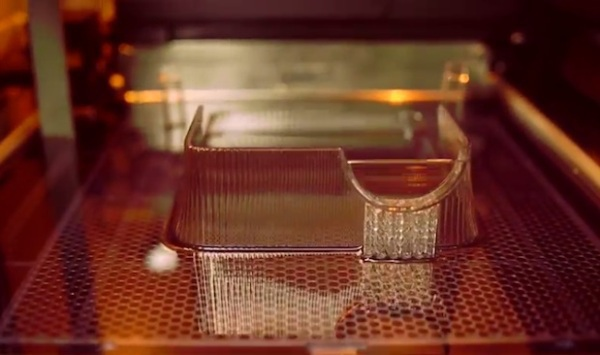
\includegraphics[scale=0.4]{./images/impression-sla.png}
\end{figure}
\newpage
\paragraph{Le procédé Polyjet} \hfill

Cette Technologie brevetée par la société israélo-américaine Objet Geometries Ltd, fonctionne aussi sur le principe de photopolymérisation.\hfill

De la même manière, l'objet sera modélisé en 3D avec un logiciel spécialisé (AutoCAD par exemple) puis son fichier envoyé à l'imprimante. Les têtes d'impressions vont alors déposer en goutte à goutte de la matière photosensible sur un support de gel, selon les coordonnées transmises par le fichier. Une fois la matière déposée, celle-ci va être exposée à un rayon ultraviolet qui va alors la durcir instantanément. L'opération sera répétée jusqu'à obtention de l'objet final, il ne restera alors plus qu'à le nettoyer. Avec une précision de l'ordre de 0,005mm il est possible de réaliser des objets avec un haut niveau de détail et des pièces d'assemblage pouvant s'imbriquer comme des engrenages.\hfill

Objet Geometries a par la suite affiné cette technique en mettant au point Polyjet Matrix. Avec 96 embouts pour chacune de ses têtes d'impression, il est possible pour l'utilisateur de combiner plusieurs matériaux différents, souples ou plus rigides. En vous permettant de créer votre propre composite, ce procédé vous offre la possibilité d'imprimer des d'objets plus variés et plus complexes.

\begin{figure}[h!]
\centering
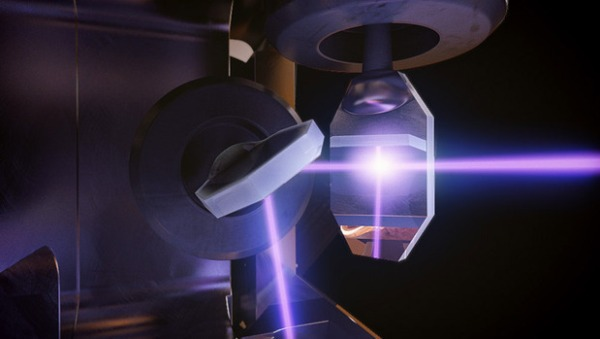
\includegraphics[scale=0.4]{./images/procede-polyjet.png}
\end{figure}
\newpage
\paragraph{Le frittage laser} \hfill

Cette technique crée par un étudiant américain dans une université du Texas en 1980, a été développée plus tard (2003) par la société allemande EOS.\hfill \

Appelée aussi SLS (Selective Laser Sintering), il s'agit également d'un processus d'impression par laser. Cette fois ci un faisceau laser très puissant va fusionner une poudre (1mm d'épaisseur) à des points très précis définis par un fichier STL que communique votre ordinateur à votre imprimante. Les particules de poudre sous l'effet de la chaleur vont alors fondre et finir par se fusionner entres elles. Une nouvelle couche de poudre fine est ensuite étalée et à nouveau durcie par le laser puis reliée à la première. Cette opération est répétée plusieurs fois jusqu'à ce que votre pièce soit finie. Ensuite, votre partie est soulevée de la poudre libre et l'objet est brossé puis sablé ou poncé à la main pour les finitions.\hfill

La poudre que l'on utilise le plus souvent pour ce type d'impression est de la polyamide. De couleur blanche ce matériau est en fait un nylon. Il va donner à votre objet une surface poreuse qui pourra d'ailleurs être repeint si vous souhaitez lui donner de la couleur. D'autres composants comme de la poudre de verre, de la céramique ou du plastique sont aussi utilisés. Souvent les fabricants utilisent un mélange de deux sortes de poudres pour obtenir des objets plus aboutis.\hfill

Sur le même principe on retrouve aussi le DMLS qui est l'abrégé de Direct Metal Laser Sintering. Ce procédé permet de réaliser des objets en métal en fusionnant cette fois une poudre de fines particules métalliques. Presque tous les métaux peuvent être utilisés, cela va du cobalt au titane en passant par l'acier et des alliages comme l'Inconel.\hfill

Même si sa précision d'impression est inférieure au SLA, le frittage laser permet de fabriquer des pièces avec un niveau de détail assez élevé (0.1mm) et à géométrie complexe. De plus la poudre restante qui n'aura pas été passée au laser pourra être réutilisée la fois suivante. Généralement les pièces obtenues avec ce processus demande davantage de finitions (ponçage, peinture, vernis...) que le SLA du fait de son rendu un peu granuleux.

\begin{figure}[h!]
\centering
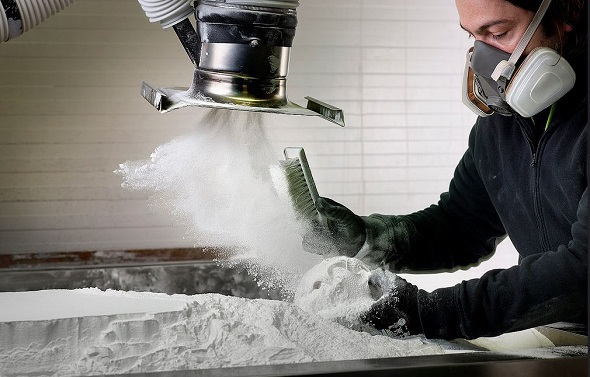
\includegraphics[scale=0.4]{./images/procede-sls.png}
\end{figure}

\begin{figure}[h!]
\centering
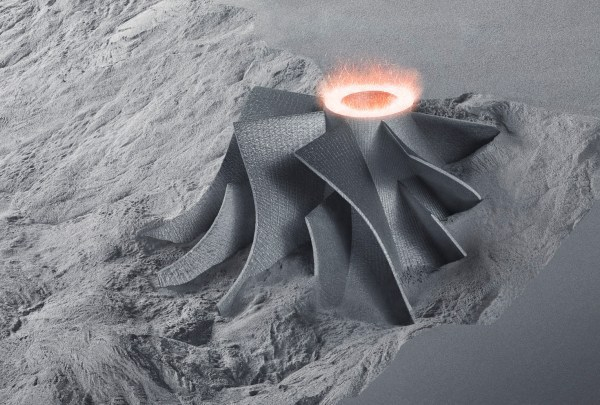
\includegraphics[scale=0.4]{./images/slm.png}
\end{figure}
\subsubsection{Agglomération de poudre par collage}
\paragraph{La 3DP} \hfill

Initialement développée en 1993 au Massachusetts à l'Institut of Technology ( MIT ) en 1993, la 3DP (Three-Dimensional Printing) constitue la base du processus d'impression 3D de Z Corporation. \hfill

Le procédé consiste en l'étalement d'une fine couche de poudre de composite sur une plateforme. La tête d'impression va alors déposer sur celle-ci de fines gouttes de glue colorées qui combinées entre elles permettent d'obtenir un large panel de couleur. La plateforme s'abaisse au fur et à mesure que les couches de poudre sont collées jusqu'à obtenir l'objet final. Pour la finition il faut aspirer l'excédent de poudre, brosser et/ou poncer la pièce, puis la chauffer pour finaliser la solidification. La 3DP a l'avantage d'être rapide et de proposer une large gamme de couleurs. Jusqu'à 6 fois moins chère qu'une imprimante SLA son prix est plus attractif malgré une précision et une qualité d'impression parfois inférieure. Parmi les inconvénients, sans traitement post-impression les pièces sont plus fragiles et leur surface est plus rugueuse. 
\begin{figure}[h!]
\centering
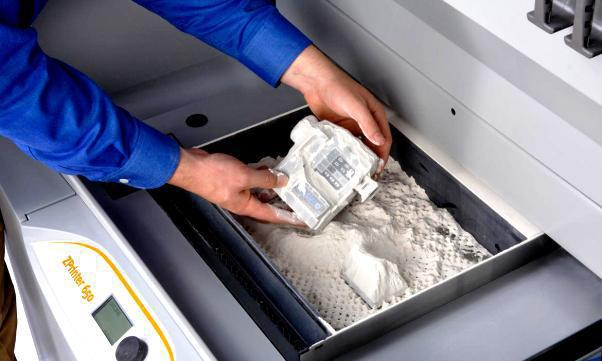
\includegraphics[scale=0.4]{./images/zprinter-650.png}
\end{figure}
\newpage
\subsection{Quelles sont les applications possibles ?}
L'impression 3D est un procédé de fabrication dont l'étendue du champ d'application reste encore sous estimé par beaucoup. Si les médias relayent de plus en plus ses exploits, pour autant le grand public et même les professionnels ignorent bien souvent tout de son réel potentiel et de ses multiples usages...\hfill

Cette technologie offre pourtant des possibilités de créations qui remettent aujourd'hui sérieusement en question notre manière de produire de nombreux objets. Grâce à la diversité de ses procédés et de ses matériaux, la fabrication additive permet déjà de fabriquer une très large gamme de produits.

\subsubsection{Prototypage}
\begin{figure}[h!]
\centering
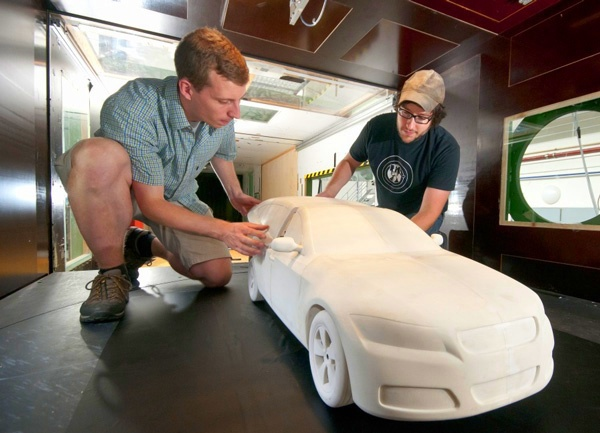
\includegraphics[scale=0.4]{./images/proto-voiture.png}
\end{figure}\hfill 

Si l'impression 3D n'est médiatisée que depuis quelques années, pour autant ce procédé ne date pas d'aujourd'hui. En effet, cette technologie trentenaire dont le 1er brevet a été déposé en 1984, est connue depuis plus de 20 ans par les industriels sous le nom de fabrication additive (fabrication par addition de couches) ou de prototypage rapide. Ce dernier terme doit son nom à l'utilisation de l'impression 3D pour la fabrication de prototypes, seule application vraiment fonctionnelle à cette époque. \hfill
\par\leavevmode\par
Un prototype désigne en fait le premier exemplaire d'un produit, une version test qui permet de vérifier sa conception et sa faisabilité avant sa production en série. De par sa fonction, il est donc non seulement produit en très petite quantité mais est aussi amené à changer souvent de caractéristiques. De ce fait la fabrication d'un prototype n'est pas adaptée à la production de masse beaucoup trop coûteuse pour de si petites quantités.\hfill

L'impression 3D présente l'avantage d'être très économique grâce à un process de conception raccourci. Contrairement aux techniques de fabrication traditionnelles (injection plastique, fraisage...), il n'y a ni d'outillage ni assemblage, ce qui rend la création plus rapide en éliminant de la main d'œuvre et de nombreux intermédiaires. Les industriels qui utilisent ce procédé peuvent passer directement de l'idée à l'objet, c'est-à-dire du modèle 3D au prototype en quelques heures et non plusieurs semaines. Cette capacité à réduire le temps et le coût de production, séduit de plus en plus d'industriels qui intègrent aujourd'hui cette technologie dans leur process de conception. \hfill

Signe fort de cet intérêt, le prototypage rapide représente plus de 70\% du marché de l'impression 3D. Parmi les industriels à faire du prototypage rapide, citons par exemple Adidas pour le prototypage de ses chaussures F50 Micoach (voir photo ci-dessous).
\begin{figure}[h!]
\centering
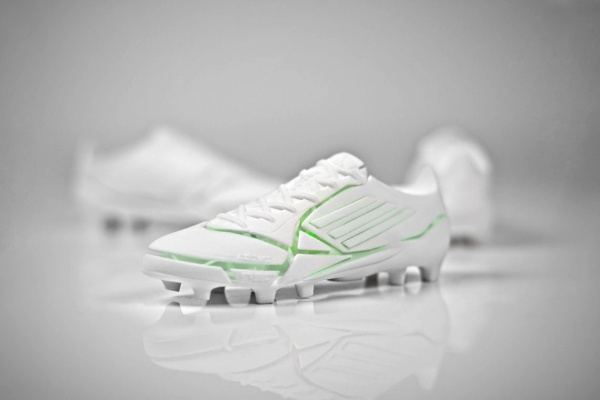
\includegraphics[scale=0.4]{./images/prototype-F50-Micoach.png}
\end{figure}

\subsubsection{Maquettes}
La fabrication de maquettes fait partie des toutes premières applications de l'impression 3D. Le plus souvent destinée à des projets architecturaux ou artistiques, la maquette est une représentation miniature, concrète et tactile, qui permet de visualiser en trois dimensions, de juger et de vérifier la faisabilité d'un projet. L'impression 3D présente de nombreux avantages par apport aux techniques traditionnelles de fabrication :
\begin{itemize}
\item Un gain de temps : quelques heures seulement avec l'impression 3D contre souvent plusieurs
jours de réalisation pour des maquettes en mousse ou en bois.
\item Plus économique : L'impression 3D est beaucoup plus économique sur les petites et moyennes
séries (jusqu'à 75\%) que les techniques classique de moulage, d'usinage ou d'assemblage.
\item Une meilleure précision : plus précise, l'impression 3D est capable de retranscrire un design au micron près et autorise des formes beaucoup plus complexes.
\item Une meilleure résistance : que ce soit l'ABS pour le procédé FDM (dépôt de fil en fusion) ou les polymères pour le frittage laser, les matériaux d'impression offrent une meilleure résistance que les matériaux traditionnels souvent plus fragiles.
\end{itemize}
\begin{figure}[h!]
\centering
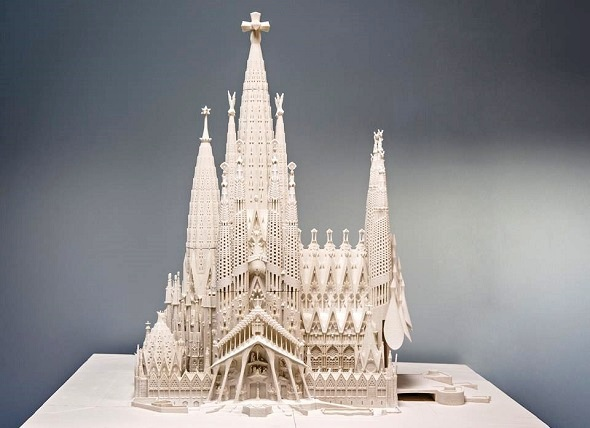
\includegraphics[scale=0.4]{./images/Maquette-imprimee-3D-Sagrada-Familia.png}
\end{figure}

\subsubsection{Outils}
L'impression 3D est également de plus en plus utilisée en pré-production. Elle intervient dans la phase de conception de pièces outils pour améliorer l'efficacité du processus de production industriel. Dans ce domaine, elle permet de faire baisser les coûts de production grâce à l'accélération du processus de fabrication des moules, des maîtres modèle ou via la fabrication directe d'outils. En effet les outillages sont généralement des pièces fabriquées en petites séries qui peuvent se révéler très complexes. Avec l'impression 3D, on peut fabriquer en s'affranchissant de toute contrainte de formes et de délais. Outre le fait de réduire le cycle de production, les moules imprimés par exemple, présentent aussi l'avantage de refroidir plus rapidement la matière injectée. \hfill

Des atouts qui ont séduit déjà nombre d'entreprises et pas des moindres, à l'image de Adidas qui a utilisé une imprimante 3D pour concevoir les moules de ses chaussures Springblades, ou encore Opel qui a fait imprimer une quarantaine d'outils (gabarits de montage par exemple) pour les lignes d'assemblages de ses véhicules Adam, Cascada et Insignia.

\begin{figure}[h!]
\centering
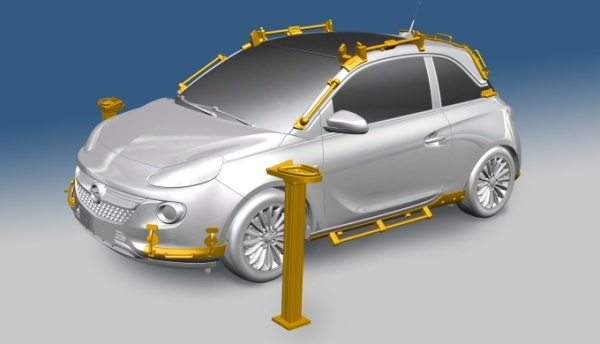
\includegraphics[scale=0.4]{./images/opel-impression-3d.png}
\end{figure}\hfill
\newpage
\subsubsection{Prothèses}
\begin{figure}[h!]
\centering
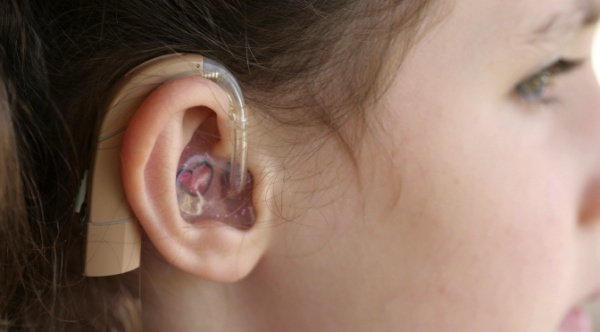
\includegraphics[scale=0.4]{./images/prothese-auditive-impression3d.png}
\end{figure}\hfill

Après l'industrie, le secteur de la santé est le plus représenté. En effet la fabrication additive est une technologie en plein essor dans le domaine médical, les fabricants de prothèses auditives et dentaires étant ceux qui utilisent aujourd'hui le plus ce procédé. Ces derniers emploient déjà massivement (depuis plus de 10 ans déjà) cette technologie qui présente l'avantage de produire des pièces sur mesures parfaitement adaptés à la morphologie du patient. Si ces dernières étaient particulièrement coûteuses à produire avec les méthodes conventionnelles, l'impression 3D a permis de faire chuter leur coût de production et de raccourcir les délais de fabrication. Certaines imprimantes 3D sont par exemple capables de produire jusqu'à 65 appareils auditifs en moins de 90 minutes... \hfill
 \par\leavevmode\par
Les laboratoires dentaires et d'orthodontie utilise de plus en plus l'impression 3D pour sa précision et sa production accrue. Selon les imprimantes 3D, il est possible de fabriquer des moulages de dents, des gouttières, des bridges ou des couronnes provisoires parfaitement ajustées à la denture du patient.\hfill
 \par\leavevmode\par
Preuve de cette utilisation massive, selon l'expert Britannique Phil Reeves, en 2010 ce sont pas moins de 10 millions de prothèses auditives, 500 000 implants dentaires et 17 millions de gouttières qui ont été imprimées en 3D dans le monde. Sans le savoir, il n'est donc pas impossible que vous portiez des objets conçus avec cette technologie...\hfill
 \par\leavevmode\par
Les dentistes utilisent également des imprimantes 3D pour concevoir des guides chirurgicaux. Une fois posés sur la denture du patient, ces derniers servent de guide pour poser différents implants.\hfill
 \par\leavevmode\par
Ces dernières années l'impression 3D s'est particulièrement illustrée dans le domaine du handicap, en permettant l'accès à des prothèses de membres (d'avant-bras et de mains) très bon marché. Ces dispositifs extrêmement coûteux (de 10 000 à 70 000 \euro) lorsqu'ils sont fabriqués avec les techniques traditionnelles, peuvent être imprimés pour quelques centaines d'euros seulement. Sous l'impulsion de Robohand, un projet philanthropique né en 2011, une dizaine de programmes associatifs (Not Impossible, E-NABLE, Bionico...) partagent aujourd'hui les plans de leurs prothèses open source, sur des plateformes de partage telles que Thingiverse. Ainsi n'importe qui dans le monde, peut télécharger le fichier et imprimer sa prothèse en y apportant ses propres modifications selon sa morphologie et ses goûts. Lorsqu'une personne n'a pas d'imprimante 3D, ces réseaux se chargent de la mettre en relation avec le bénévole le plus proche.

\begin{figure}[h!]
\centering
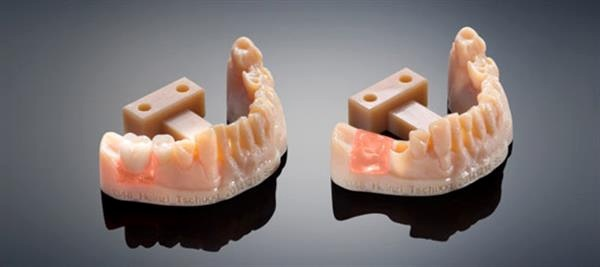
\includegraphics[scale=0.4]{./images/prothesedentaire.png}
\end{figure}

\begin{figure}[h!]
\centering
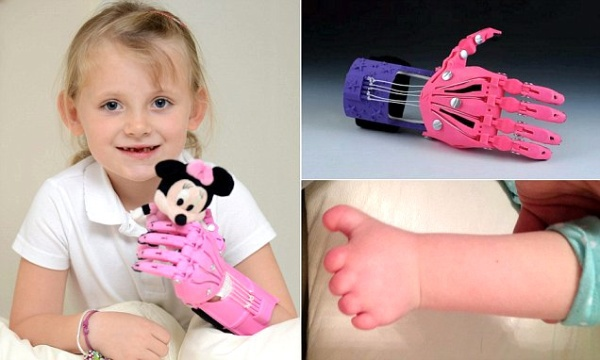
\includegraphics[scale=0.4]{./images/HarleyFraser.png}
\caption{En 2014 – Harley Fraser, petit fille britannique de 5 ans équipée d'une prothèse de main imprimée en 3D}
\end{figure}
\newpage
\subsubsection{Implants}
Perçue comme l'une des meilleures voies d'amélioration de l'efficacité\hfill \break thérapeutique, la fabrication additive permet aujourd'hui de fabriquer des implants médicaux sur-mesure. Couplée à l'imagerie médicale (via scanner, IRM ou échographie), celle-ci permet de reproduire à l'identique les caractéristiques anatomiques du patient pour concevoir des dispositifs médicaux implantables parfaitement adaptés à sa morphologie.\hfill
 \par\leavevmode\par
C'est en 2012 que le premier implant à été fabriqué selon ce procédé. Il s'agissait d'une mandibule de mâchoire en titane implantée sur une femme de 83 ans atteinte d'ostéomyélite.\hfill
 \par\leavevmode\par
En 2014, le français MEDICREA a implanté le premier implant vertébral imprimé en 3D au monde. Un
dispositif sur-mesure faisant corps avec la colonne du patient et prenant parfaitement appui sur les plateaux vertébraux. Signe fort de l'intérêt grandissant pour cette technique, plus de 20\nobreak 000 implants médicaux ont été imprimés entre 2007 et 2014.

\begin{figure}[h!]
\centering
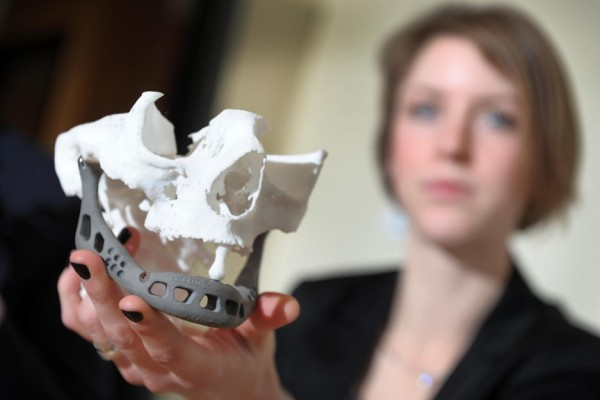
\includegraphics[scale=0.4]{./images/Machoire.png}
\end{figure}
\newpage
\subsubsection{Modèles chirurgicaux}
La fabrication de modèles chirurgicaux par impression 3D fait partie des usages les plus en vogue dans le milieu médical. Il s'agit en fait de la reproduction d'un organe ou d'un os destiné le plus souvent à préparer une intervention. Ce modèle très fidèle à l'original, permet au chirurgien de mieux visualiser la zone qu'il va opérer et de s'entraîner avant l'opération.\hfill
 \par\leavevmode\par
Il permet de réduire la durée des interventions et par conséquent ses risques et les effets post opératoires. Ces modèles 3D ont déjà fait plusieurs fois leur preuve, notamment pour les opérations complexes requérant un geste opératoire très précis.\hfill
 \par\leavevmode\par
En 2014, un nourrisson dénommé Roland Lian Cung Bawi, alors atteint de malformations cardiaques, avait pu être sauvé grâce à une reproduction imprimée en 3D de son cœur malade.\hfill
 \par\leavevmode\par
Cette même année, le Boston Children's Hospital avait opéré avec succès un bébé épileptique, en fabriquant une réplique très fidèle de son cerveau par impression 3D.\hfill
 \par\leavevmode\par
Ces modèles 3D médicaux représentent aussi un outil pédagogique très \hfill \break intéressant pour les étudiants en médecine et les patients.

\begin{figure}[h!]
\centering
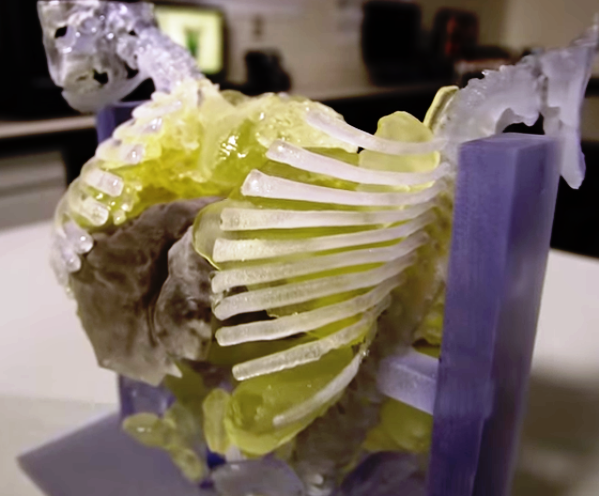
\includegraphics[scale=0.4]{./images/Modele-chirurgical.png}
\caption{Modèle chirurgical d'un thorax de soeurs siamoises}
\end{figure}
\newpage

\subsubsection{Alimentaire}
\begin{figure}[h!]
\centering
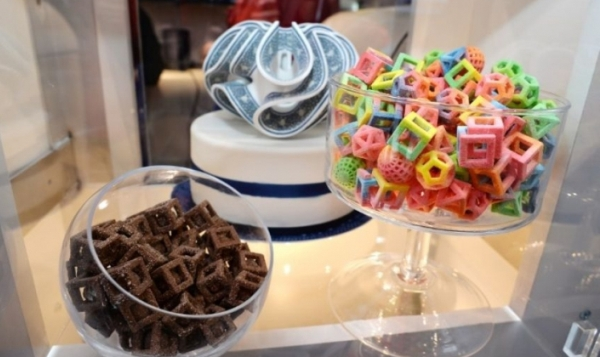
\includegraphics[scale=0.4]{./images/bonbons.png}
\end{figure}\hfill

Si on associe rarement impression 3D et alimentation, ce domaine est pourtant lui aussi concerné par cette technologie. Le procédé employé pour les aliments, s'appuie sur celui du FDM qui consiste habituellement à superposer des couches de matières plastiques en fusion.\hfill
 \par\leavevmode\par
Pour une imprimante 3D alimentaire, la différence se situe au niveau de la buse qui est remplacée par une seringue d'où va être extrudée la matière. Dans le cas de l'impression 3D de nourriture, la machine ne créé pas la matière, elle permet « juste » de lui donner la forme que l'on souhaite. Les bénéfices de l'impression 3D dans ce domaine, résident essentiellement dans sa capacité à réaliser des formes complexes (pièces en sucre ou chocolat), et à imprimer des aliments à la texture modifiée, notamment pour les personnes âgées souffrant de troubles de déglutition et de mastication. On pourrait également créer des plats personnalisées, adaptés aux besoins nutritionnels, carences ou allergies de chaque
personne.\hfill
 \par\leavevmode\par
Parmi les cas les plus illustres dans ce domaine, il y a celui-ci de la NASA qui a été l'un des premiers à s'intéresser à ce procédé. Souhaitant améliorer les conditions d'alimentation de ses astronautes lassés de leurs poudres lyophilisées, l'administration américaine a investit pas moins de 125000 \$ pour développer une imprimante 3D alimentaire. Fabriquée à partir du modèle Reprap Mendel 3D, cette machine encore à l'état de prototype, est déjà capable d'imprimer du chocolat et même des pizzas avec des premiers tests très prometteurs. Cette même année (2013) l'entreprise espagnole Natural Machines a dévoilé sa Foodini, une imprimante 3D destinée à fabriquer des pâtes à pizza ou à quiches qui peuvent ensuite être cuites au four. La machine est désormais disponible en pré commande.\hfill
 \par\leavevmode\par
Parmi les précurseurs dans ce domaine, citons également Sugar Labs, une compagnie américaine basée à Los Angeles qui a conçu la première imprimante 3D capable d'imprimer des pièces de sucre. La société a été rachetée en 2013 par son compatriote 3D Systems, qui s'est appuyé sur leur technologie pour mettre au point la série Chef Jet. Il s'agit d'une gamme d'imprimantes 3D alimentaires destinée aux particuliers et aux professionnels pour la réalisation de confiseries, de nappages ou de décors en sucre...\hfill 
 \par\leavevmode\par
En matière d'impression 3D de chocolat, le précurseur s'appelle Choc Edge , une compagnie britannique fondée en 2012 par deux chercheurs de l'université d'Exeter. Ces derniers ont mis au point la Choc Creator, première imprimante 3D capable de fabriquer des pièces en chocolat. Parmi ses concurrents, citons l'australien Solidea et sa Chocabyte ou plus récemment l'américain 3D Systems et sa Cocojet.

\begin{figure}[h!]
\centering
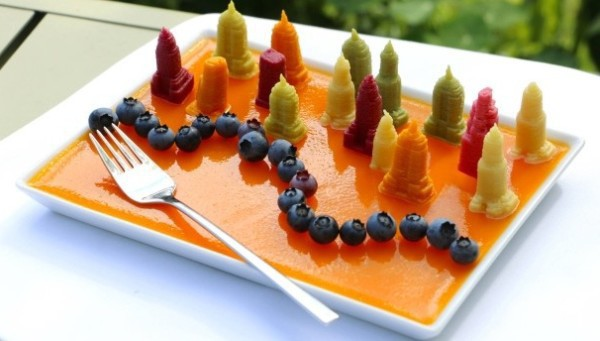
\includegraphics[scale=0.4]{./images/alimentation.png}
\end{figure}\hfill

\subsubsection{Mode}

Si l'impression 3D est encore balbutiante dans le secteur de la mode, de nombreux créateurs et designers ont déjà intégré ce procédé dans leur processus créatif. Du fait de son potentiel de personnalisation, cette technologie est particulièrement légitime dans ce domaine. En scannant les différentes parties du corps, il est en effet possible de créer un vêtement (robe, veste, chaussure...) sur-mesure parfaitement adapté à la morphologie de la personne. La marque Continiuum Fashion par exemple, propose des chaussures, des bikinis et divers accessoires entièrement imprimés en 3D.\hfill
 \par\leavevmode\par
Les créateurs de mode voient également dans l'impression 3D, un moyen de créer des prototypes à moindre coût et de créer des formes très complexes habituellement impossibles à réaliser avec les techniques traditionnelles. Parmi les créations les plus étonnantes, mentionnons la magnifique Parure Quixotic Divinity du designer Joshua Harker, la robe très sexy de Michael Schmidt et Francis Bitonti portée par Dita Von Teese (photo ci-dessous) ou encore la Robe araignée de Anouk Wipprecht.

\begin{figure}[h!]
\centering
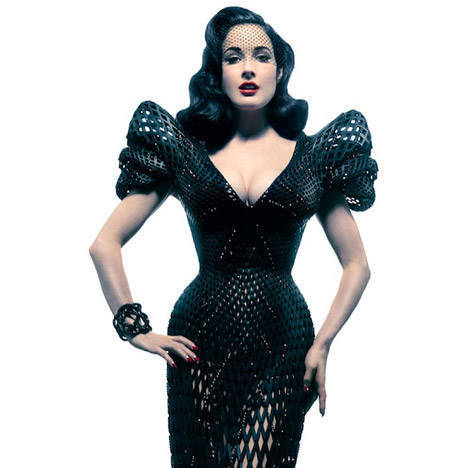
\includegraphics[scale=0.4]{./images/Mode.png}
\end{figure}\hfill
\newpage

\subsubsection{Habitat}

Déjà employée par les architectes pour la fabrication de maquettes de villes ou de bâtiments, l'impression 3D est désormais utilisée pour la construction de maisons à taille réelle. Le précurseur en la matière s'appelle Contour Crafting, une entreprise californienne à vocation humanitaire qui a mis au point un procédé d'impression 3D béton. La machine en question se présente sous la forme d'un gros extrudeur, qui se déplace sur un rail et superpose des couches de ciment composite, comme pourrait le faire une imprimante 3D FDM de bureau. Si la machine n'est pas encore tout à fait au point, d'autres
entreprises ont pris une longueur d'avance et commercialisent déjà la leur. C'est le cas de Winsun , une société chinoise qui a développé une imprimante 3D capable de fabriquer 10 maisons en l'espace de 24 h (et même des immeubles pour un coût de 4300 \euro{} seulement...). BetAbram est actuellement son concurrent le plus sérieux. Cette société slovène commercialise déjà 3 modèles d'imprimantes 3D avec des prix compris entre 12 000 et 32 000 \euro{} pour des volumes d'impression allant de 12m$^{2}$ à 144m$^{2}$.

\begin{figure}[h!]
\centering
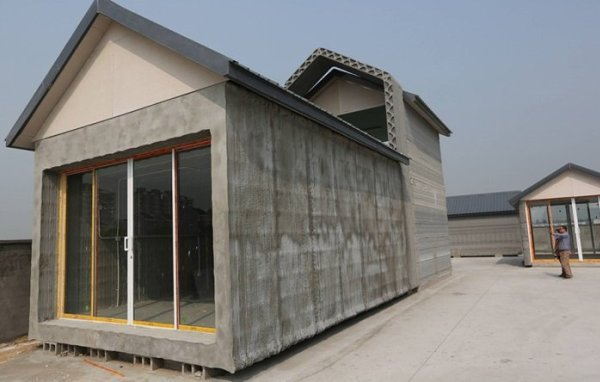
\includegraphics[scale=0.4]{./images/maison.png}
\end{figure}\hfill
\newpage

\subsubsection{Tissus Biologiques}

On pourrait croire à de la science fiction et pourtant... La bioimpression ou « bioprinting » qui correspond à l'impression 3D de tissus biologiques, est aujourd'hui une réalité. Le précurseur dans ce domaine s'appelle Organavo , une entreprise américaine qui a mis au point une imprimante 3D très particulière, capable d'imprimer des cellules vivantes. Baptisée NovoGen MMX Bioprinter, cette machine fonctionne sous un procédé similaire à la technologie FDM (superposition de matière fondue) utilisées par les imprimantes 3D de bureau. Les tissus sont imprimés à partir d'un matériau de support appelé hydrogel, dans lequel sont injectés des cellules souches qui fusionnent ensuite entre elles jusqu'à obtenir les fonctions biologiques désirées. Parmi les acteurs majeurs du bioprinting, citons également Poietis, une société française qui a mis au point un système de Bioimpression 4D par laser, unique au monde. Concernant l'impression d'organes, qui plus est viables et transplantables, c'est un domaine d'application pour le moment beaucoup trop complexe. Même si plusieurs laboratoires
travaillent dessus, cela relève pour le moment du domaine du rêve.

\begin{figure}[h!]
\centering
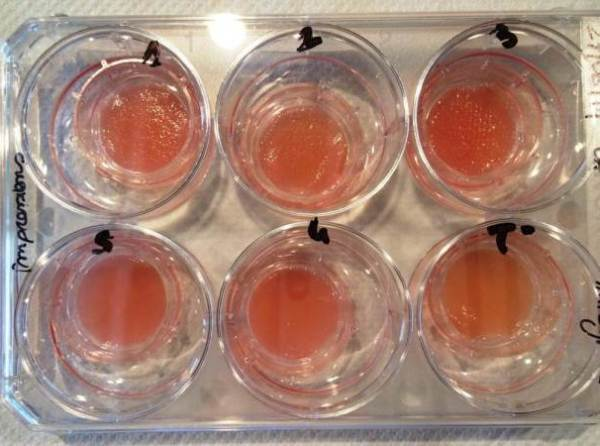
\includegraphics[scale=0.4]{./images/tissus.png}
\end{figure}\hfill
\newpage

\subsubsection{Bijoux}

Avec l'odontologie (dentisterie), la bijouterie est le domaine qui recours le plus à l'impression 3D... à tel point qu'il n'utilise quasiment plus que ce procédé. Bien que pour le moment il ne soit pas possible d'imprimer directement des métaux précieux tels que l'or ou l'argent, cette technologie permet de fabriquer des moules à cire perdue. Ces derniers se destinent à donner la forme au moule final (moule réfractaire) dans lesquels sont coulés les métaux en fusion. Aujourd'hui de nombreux constructeurs proposent des gammes d'imprimantes 3D spécialisées dans la fabrication de moules à cire perdue.
L'impression 3D offre plusieurs avantages comme la diminution des temps de fabrications des modèles, mais aussi une excellente finition. Pour les métaux moins nobles tels que l'acier ou le titane, les bijoux peuvent être directement imprimés via des techniques d'impression par laser comme le DMLS (fusion de poudres métalliques).

\begin{figure}[h!]
\centering
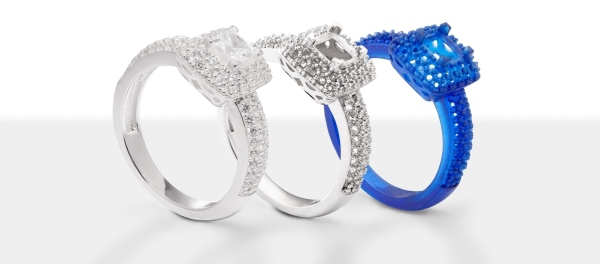
\includegraphics[scale=0.4]{./images/bijoux.png}
\end{figure}\hfill
\newpage

\subsubsection{Accessoires et objets du quotidien}

\begin{figure}[h!]
\centering
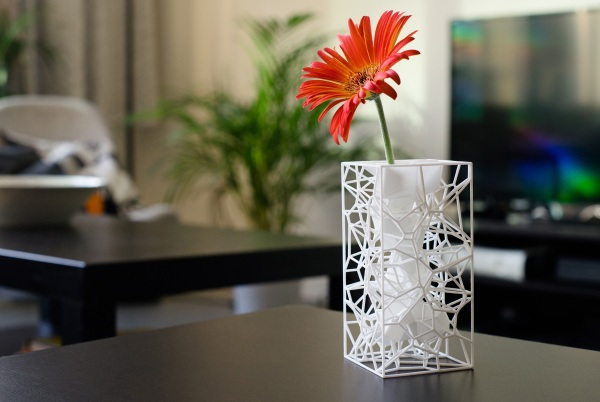
\includegraphics[scale=0.4]{./images/vase-design.png}
\end{figure}\hfill 

Outre ses applications dans le domaine industriel, l'impression 3D s'adresse plus directement aux particuliers via la fabrication d'accessoires personnalisés. Ainsi certains services tels que Sculpteo, propose par exemple d'imprimer des coques de téléphone portable, customisables presque à volonté. Le client a la possibilité de personnaliser sa coque de protection en y intégrant par exemple son prénom, le relief d'un paysage voir même son propre visage grâce à différents outils et applications proposées sur le site.\hfill
 \par\leavevmode\par
On peut fabriquer toute sorte d'objets avec une imprimante 3D de bureau, comme par exemple des prototypes, des maquettes ou certaines pièces de réparation. Le grand public l'emploie surtout pour imprimer des objets du quotidien. Les impressions les plus courantes concernent généralement des objets décoratifs comme des vases par exemple, mais aussi des accessoires tels que des presse-agrume, des coquetiers, des porte-crayon ou encore des portes-clef... Grâce à l'impression 3D, l'utilisateur peut réaliser des objets personnalisés pour quelques centimes ou quelques euros seulement.

\begin{figure}[h!]
\centering
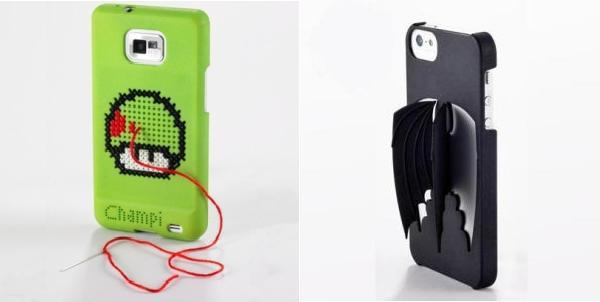
\includegraphics[scale=0.4]{./images/coque.png}
\end{figure}\hfill

\subsubsection{Artistique}

Les artistes se sont aussi très vite emparés de cette technologie pour créer des sculptures aux formes très diverses et très complexes. L'impression 3D a créé un nouveau processus de création, une nouvelle forme d'expression artistique. Le modèle numérique étant quelque chose de malléable, le processus créatif du sculpteur est très différent. Il peut revenir en arrière, rectifier son modèle, le retravailler et expérimenter à l'infini avant d'aboutir à la pièce parfaite. Ainsi l'impression 3D a donné naissance à une nouvelle esthétique mais surtout une nouvelle forme d'art : la sculpture numérique.\hfill
 \par\leavevmode\par
À la fois artiste et ingénieur, Joshua Harker fait partie des pionniers dans ce domaine. Cet américain a développé une technologie d'impression 3D qui lui permet de créer des pièces artistiques d'une finesse et d'une complexité incroyables, à l'image du magnifique bouquet de fleur ci-dessous.

\begin{figure}[h!]
\centering
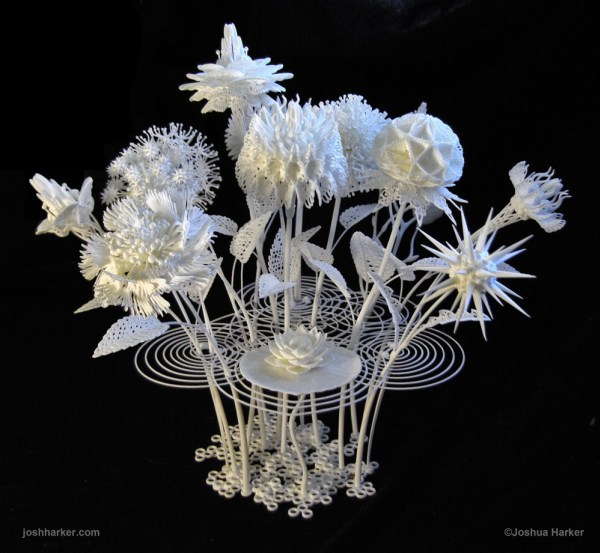
\includegraphics[scale=0.4]{./images/artistique.png}
\end{figure}\hfill

\subsubsection{Figurines}

S'il est bien un objet qui symbolise à lui seul le potentiel de personnalisation de l'impression 3D, c'est la figurine. Il est en effet possible d'imprimer des statuettes personnalisées extrêmement réalistes, reproduisant à la perfection les moindres détails d'un visage et d'un vêtement. Les premiers services spécialisés sont apparus en 2012, proposant d'imprimer des figurines selon différents procédés : soit à partir de photos, soit à partir d'un scan de l'individu. Les figurines sont imprimées sur des poudres de céramique ou de polymère. Le client peut commander sa propre réplique miniature, ou incarner un personnage en combinant sa tête au corps d'un super héros (cowboy, footballeur, avocat...).

\begin{figure}[h!]
\centering
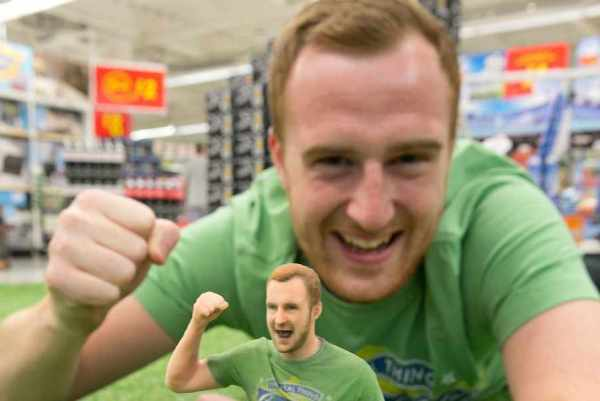
\includegraphics[scale=0.4]{./images/figurine-scannee.png}
\end{figure}\hfill 
\newpage

\subsection{Quels matériaux pour imprimer en 3D ?}


\begin{figure}[h!]
\centering
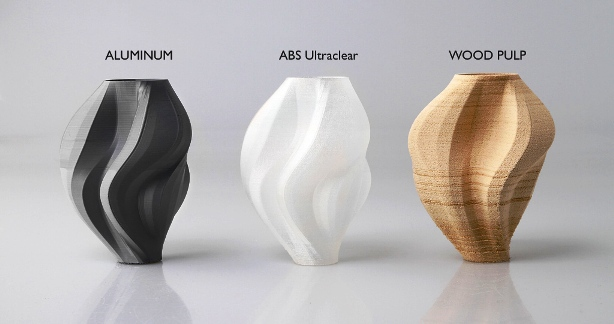
\includegraphics[scale=0.4]{./images/materiaux-impression.png}
\end{figure}\hfill

Certains pourraient croire que le plastique est le seul matériau utilisé dans l'impression 3D, hors cette technologie offre aujourd'hui un très large panel de consommables ! En effet, chaque procédé d'impression 3D fonctionne avec son propre type de matériau. Ainsi la plupart des imprimantes 3D de type FDM par exemple, sont compatibles avec des filaments plastiques, alors que les machines fonctionnant selon la technologie SLA (stéréolithographie) impriment à partir de résines. \hfill 
 \par\leavevmode\par
On distingue 2 grandes familles de matériaux à savoir les plastiques et les métaux. À cela s'ajoute les céramiques (silice, alumine, plâtre...) et les matières organiques (cires, tissus et cellules). Nous allons faire ici le point sur les caractéristiques et les utilisations des principaux matériaux utilisés pour imprimer en 3D.

\subsubsection{Les matériaux plastiques}

Parmi les plastiques les plus utilisés pour l'impression 3D FDM (dépôt de plastique fondu), il y a 2 consommables dominants : le PLA et l'ABS qui sont des polymères et des thermoplastiques qui deviennent mous et malléables lorsqu'ils sont chauffés et qui reviennent à un état solide lorsqu'il sont refroidis.

\paragraph{PLA} \hfill

Il est le consommable le plus couramment utilisé pour les imprimantes personnelles qui fonctionnent par dépôt de fil.\hfill 
 \par\leavevmode\par
Écologique car d'origine végétale (amidon de maïs, racine de manioc et betterave), ce filament est biodégradable, non toxique et sa fusion dégage une légère odeur sucrée. Si le PLA est pur et que l'extrudeur de l'appareil est en acier inoxydable, alors celui-ci peut être utilisé pour imprimer des objets destinés à être en contact avec des aliments tels que des bols ou des tasses par exemple.\hfill  \par\leavevmode\par
Une bobine de 1kg de PLA de 1,75 mm mesure en moyenne 330 mètres et 115 mètres en 3mm.\hfill 
 \par\leavevmode\par
\textbf{Température d'impression} : entre 190 et 210\degres C / Plateau chauffant optionnel\hfill

\textbf{Densité} : 1,25g/cm$^{3}$\hfill

\textbf{Points forts} : Ne dégage pas de mauvaise odeur et facile à imprimer\hfill

\textbf{Points faibles} : Sensible à l'humidité et à la chaleur\hfill
 \par\leavevmode\par
\fbox{
\begin{minipage}{1\textwidth}
il faut compter entre 30\euro{} et 60\euro{} la bobine de 1 kg. Le prix varie en fonction de la couleur, de la marque et s'il s'agit ou non d'un filament propriétaire car certaines imprimantes fonctionnent avec leurs propres matériaux.
\end{minipage}}
 \par\leavevmode\par
\paragraph{ABS} \hfill 

Fabriqué à base de pétrole, il s'agit du matériau le plus polyvalent car compatible avec presque toutes les imprimantes 3D, y compris les dérivés de RepRap et ceux de MakerBot, Ultimaker, Bits de Bytes, Airwolf3D, Makergear, Printrbot, Bukobot... L'ABS qui est soluble dans l'acétone permet de souder les pièces métalliques avec une goutte ou deux, ou de lisser et créer un effet brillant par brossage ou trempage pièces entières dans l'acétone. Sa force, sa souplesse et sa meilleure résistance à la température font de lui le matériau préféré pour les ingénieurs, et les applications professionnelles.\hfill
 \par\leavevmode\par
Une bobine de 1kg d'ABS de 1,75 mm mesure en moyenne 410 mètres et 140 mètres en 3 mm.\hfill
 \par\leavevmode\par
\textbf{Température d'impression} : entre 220 et 260 \degres C / Plateau chauffant entre 60 et 110\degres C\hfill

\textbf{Densité} : 1,01g/cm$^{3}$\hfill

\textbf{Points forts} : Matériau polyvalent et particulièrement résistant, supporte bien les écarts de température.\hfill

\textbf{Points faibles} : Odeurs pendant l'impression et parfois sujet au warping (décollement des bords de la
pièce)\hfill
 \par\leavevmode\par
\fbox{
\begin{minipage}{1\textwidth}
il faut compter entre 30\euro{} et 60\euro{} la bobine de 1 kg. Le prix varie en fonction de la couleur, de la marque et s'il s'agit ou non d'un filament propriétaire car certaines imprimantes fonctionnent avec leurs propres matériaux. \end{minipage}
}
\newpage
\subsubsection{PVA et HIPS : Les matériaux de support}

Pour une impression 3D de type FDM (dépôt de matière fondue), il faudra prévoir ce que l'on appelle un raft (ou ratier). Il s'agit d'un support qui permet de soutenir la pièce sur le plateau pendant l'impression pour qu'elle reste stable. Celui-ci se présente sous la forme d'une grille qui permet une meilleure accroche, ou d'une sorte d'échafaudage afin de soutenir certains éléments tels que le bras d'une figurine ou la base d'une fusée. Les matériaux les plus utilisés sont le PVA et l'HIPS (high-impact polystyrene) qui tous deux peuvent se dissoudre dans de l'eau ou avec du D-Limonene (un solvant) en l'espace de 24h. Ce dernier s'utilise avec de l'ABS qui possède les mêmes températures d'extrusion et de plateau, de ce fait ce matériau ne concerne que les imprimantes 3D à double extrudeur.\hfill
 \par\leavevmode\par
\textbf{Température d'impression du PVA} : entre 190 et 210\degres C / plateau chauffant optionnel\hfill

\textbf{Points forts} : facile à imprimer et inodore\hfill

\textbf{Points faibles} : sensible à l'humidité\hfill 

\textbf{Température d'impression de l'HIPS} : entre 220 et 260\degres C / plateau chauffant entre 60 et 110\degres C\hfill 

\textbf{Points forts} : Bonne finition et généralement moins cher que le PVA\hfill

\textbf{Points faibles} : Parfois sujet au warping\hfill 
 \par\leavevmode\par
\fbox{
\begin{minipage}{1\textwidth}
Environ 35\euro{} la bobine de 500g pour le PVA et 25\euro{} le kg pour le HIPS
\end{minipage}
}

\begin{figure}[h!]
\centering
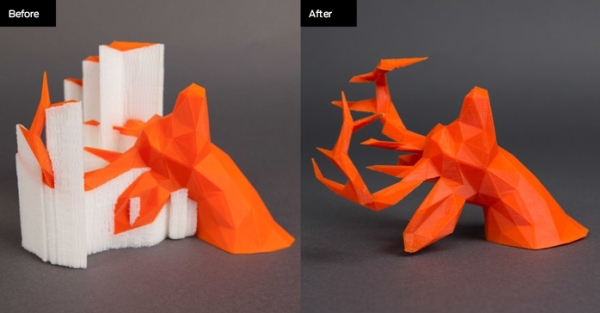
\includegraphics[scale=0.4]{./images/raft-cerf.png}
\end{figure}\hfill
\newpage

\subsubsection{La poudre de polyamide}
Ce matériau sert par exemple à imprimer des prototypes en plastique blanc via un procédé appelé frittage laser.\hfill
 \par\leavevmode\par
Comment ça marche ?\hfill
 \par\leavevmode\par
Un faisceau laser sculpte votre objet dans de la poudre de polyamide dont les grains se fusionnent et se solidifient sous l'effet de la chaleur. Les pièces peuvent être ensuite colorées en les plongeant dans un bain de teinture adapté. Le polissage permet de finir votre pièce. Cette poudre offre un grand niveau de détail et donne à vos pièces un aspect sableux, granuleux et légèrement poreux. Surtout utilisée pour la fabrication de mécanismes et d'engrenages, elle est néanmoins compatible pour des objets à contacts alimentaires.\hfill
 \par\leavevmode\par
\fbox{
\begin{minipage}{1\textwidth}
Entre 50 et 100\euro{} le kg
\end{minipage}
}

\begin{figure}[h!]
\centering
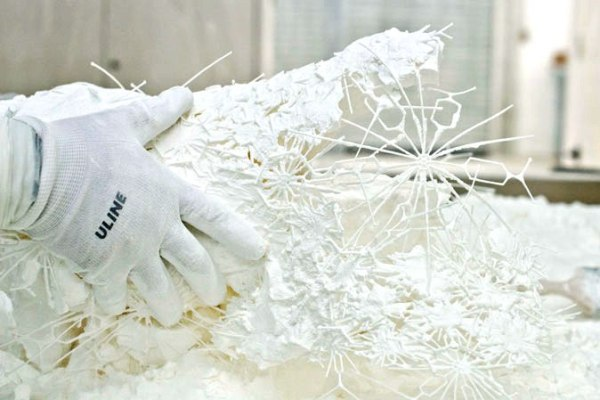
\includegraphics[scale=0.4]{./images/poudre-plastique.png}
\end{figure}\hfill
\newpage
\subsubsection{L'alumide}
\begin{figure}[h!]
\centering
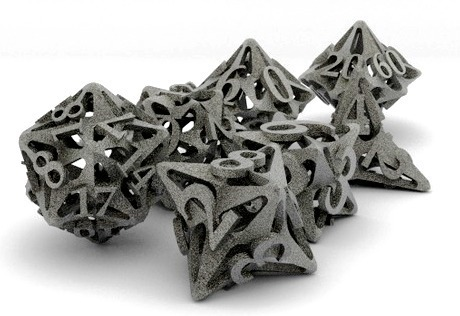
\includegraphics[scale=0.4]{./images/alumide.png}
\end{figure}\hfill
 \par\leavevmode\par
L'alumide est un mélange de polyamide et d'aluminium. Ce matériau offre l'avantage de pouvoir réaliser des pièces à la fois très solides et très flexibles avec une importante résistance à la chaleur. D'un aspect proche du métal, son impression se fait par frittage laser avec des particules d'alumine de 60 micromètres. Les objets imprimés avec ce genre de matières nécessitent ensuite divers finitions telles que le polissage ou le meulage.\hfill

\subsubsection{La résine liquide}
La résine est un polymère liquide photosensible. L'impression avec ce matériau consiste en un dépôt successif de couches qui sont immédiatement solidifiées par UV. Votre pièce prend alors les allures d'une pièce plastique rigide et lisse. La résine est à la base blanche ou noire. Cependant, vous pouvez aussi vous fournir en résine colorées. Un large éventail de couleurs est disponible parmi lesquelles figurent le bleu thalassa, le rose fluo, le jaune pâle, le rouge intense et le gris perle. Au total dix couleurs sont à votre disposition. Contrairement au polyamide, vous n'avez pas à plonger la pièce dans un bain de teinture. Par ce procédé, la pièce imprimée est colorée directement selon vos souhaits impliquant parfois une perte de détails. \hfill
 \par\leavevmode\par
\fbox{
\begin{minipage}{1\textwidth}
Le prix de ces résines est très variable : entre 200\euro{} et 600\euro{} le litre. (pour l'imprimante Form1 de Formlabs par exemple comptez environ 110\euro{} la recharge de 1L.)
\end{minipage}
}

\begin{figure}[h!]
\centering
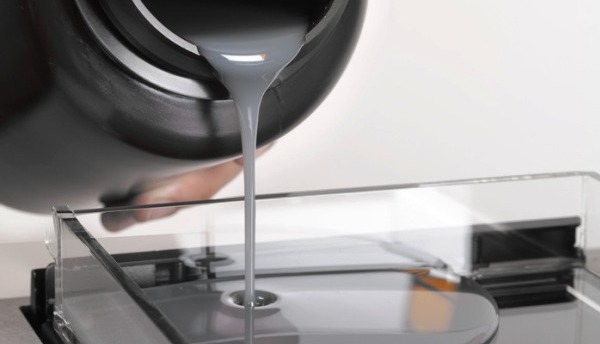
\includegraphics[scale=0.4]{./images/resine.png}
\end{figure}\hfill
\newpage

\subsubsection{La cire}
\begin{figure}[h!]
\centering
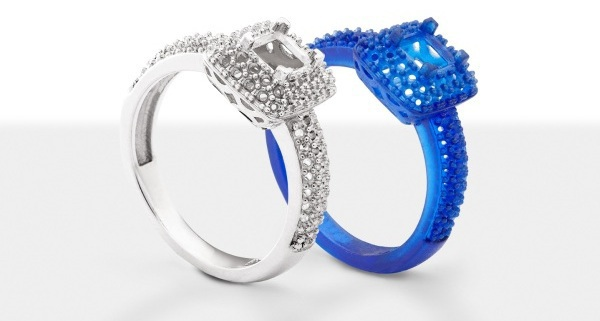
\includegraphics[scale=0.4]{./images/cire.png}
\end{figure}\hfill
 \par\leavevmode\par
La cire est composée de polymère et fond comme les autres plastiques. Ce matériau est principalement utilisé en bijouterie et en dentisterie pour la création de moules où son ensuite coulés d'autres matériaux comme du métal ou de la céramique.\hfill
 \par\leavevmode\par
Ce consommable à l'avantage de produire des pièces plus précises qu'avec les méthodes traditionnelles. Il confère aux pièces un aspect lisse sans porosité en limitant les craquelures et permet de reproduire des produits fins à l'image des alvéoles d'un nid d'abeilles. Le rendu est quasi-parfait. La solidité et sa souplesse sont ses points faibles.\hfill
 \par\leavevmode\par
L'une des cires les plus connues du marché est la Visijet Prowax. De couleur bleue, cette résine calcinable permet de fabriquer des moules pour la fonderie. Citons également la Dentcast qui se destine aux moules dentaires.
\newpage

\subsubsection{Les métaux}
\begin{figure}[h!]
\centering
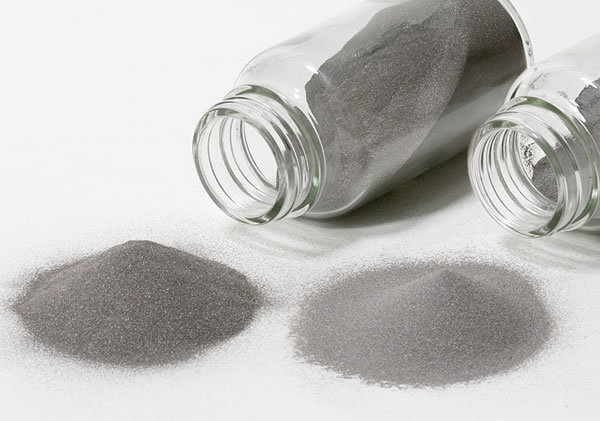
\includegraphics[scale=0.4]{./images/poudre-metallique.png}
\end{figure}\hfill
 \par\leavevmode\par
Après les plastiques, les métaux sont les matériaux les plus employés en impression 3D et essentiellement par les industriels. En tête des utilisations, on retrouve le titane et l'acier inoxydable (inox), viennent ensuite l'aluminium, le cobalt, le fer et les métaux précieux tels que le bronze, l'argent et l'or. La fabrication additive à cette capacité à pouvoir produire des pièces métalliques aux géométries plus complexes qu'avec les techniques de fabrication soustractives telles que le fraisage ou par moulage.\hfill
 \par\leavevmode\par
Le plus souvent les objets en métal sont imprimées à partir de poudres métalliques fusionnées avec un laser (procédé DMLS). Ces pièces ont aussi l'avantage d'être plus légères que des pièces traditionnelles, en étant tout aussi résistantes voir même plus. Des propriétés physiques très intéressantes donc pour les constructeurs aéronautiques ou de l'automobile par exemple, à la recherche de matériaux toujours plus légers et résistants.
\newpage
\subsubsection{L'acier inoxydable}
\begin{figure}[h!]
\centering
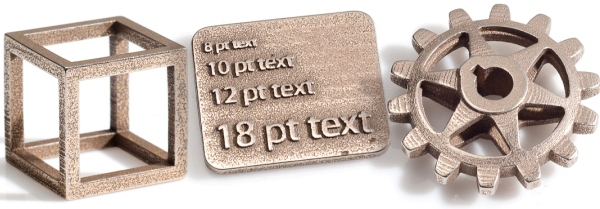
\includegraphics[scale=0.4]{./images/acier-inoxydable.png}
\end{figure}\hfill
 \par\leavevmode\par
Ce matériau plus connu sous l'appellation « d'inox » a été le premier métal à être commercialisé pour la fabrication additive. Comme son nom le suggère, il possède des propriétés mécaniques de haute résistance à la corrosion. Parmi les plus connus on peut citer le MS1, le PH1 ou le StainlessSteel GP1 du constructeur EOS, une poudre fine d'acier inoxydable réputée pour sa grande résistance à la corrosion et son excellente ductilité (capacité à se déformer sans rompre) sans aucun traitement ultérieur.\hfill
 \par\leavevmode\par
\fbox{
\begin{minipage}{1\textwidth}
Entre 90 et 200\euro{} le kg.
\end{minipage}}

\subsubsection{L'acier d'outillage Maraging}

\begin{figure}[h!]
\centering
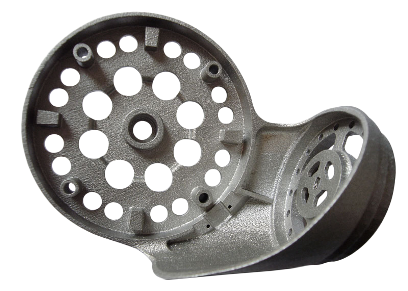
\includegraphics[scale=0.4]{./images/acier-outillage.png}
\end{figure}\hfill
 \par\leavevmode\par
Il s'agit d'un acier inoxydable martensitique, sous groupe des aciers inoxydables se caractérisant par une grande solidité et dureté, obtenues après un traitement ultérieur thermique. Ce matériau se destine avant tout à la fabrication d'outillage rapide (découpage, extrusion...) et de moules dans les domaines de l'aéronautique, l'astronautique et l'automobile. Là encore on peut citer EOS avec son acier martensitique MS1 capable de produire des pièces d'une résolution supérieure à celui de l'acier d'outillage SLS A6.

\subsubsection{Le Titane}
\begin{figure}[h!]
\centering
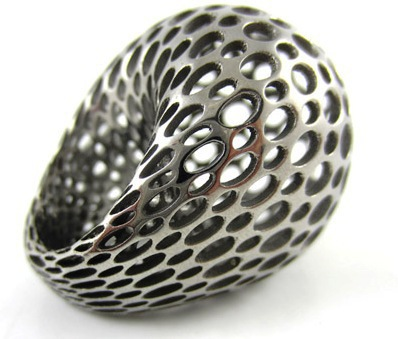
\includegraphics[scale=0.4]{./images/titane.png}
\end{figure}\hfill
 \par\leavevmode\par
Les pièces imprimées à partir de titane ou de ses alliages sont réputées pour leur légèreté, leur solidité et leur résistance à la corrosion très élevée. Les techniques traditionnelles appliquées à ce matériau ont l'inconvénient d'être coûteuses et moins fiable que la fabrication additive. En effet lorsque l'on soude une pièce en titane par exemple, des impuretés ont tendance à venir s'y déposer, fragilisant ainsi celle-ci. Le titane est par ailleurs un métal qui refroidit très rapidement, il nécessite donc l'utilisation d'outils particulièrement chers.\hfill
 \par\leavevmode\par
La fabrication additive est donc de plus en plus employé lorsqu'il s'agit de travailler ce matériau, les plus gros utilisateurs étant les secteurs de l'automobile, l'aéronautique et de la médecine. Les alliages de titane tels que le Ti6Al4V sont plus solides que matériau original pur. Cet alliage biocompatible trouve notamment des applications dans la médecine. Il est utilisé par exemple pour fabriquer d'implants en titane sur mesure, sa porosité naturelle permettant aux cellules osseuses de le coloniser efficacement.\hfill
 \par\leavevmode\par
\fbox{
\begin{minipage}{1\textwidth}
Entre 400 et 500\euro{} le kg
\end{minipage}}
\newpage

\subsubsection{L'aluminium}
\begin{figure}[h!]
\centering
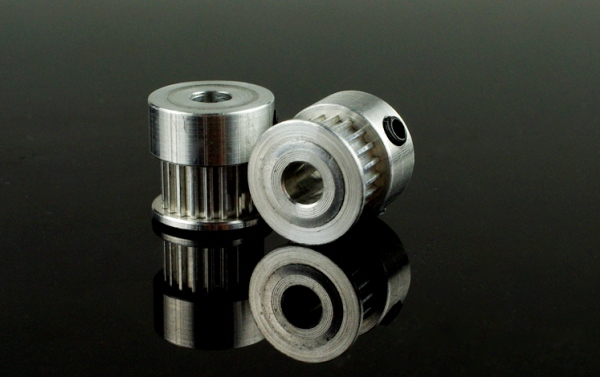
\includegraphics[scale=0.3]{./images/aluminium.png}
\end{figure}\hfill
 \par\leavevmode\par
Dans cette catégorie, on retrouve l'AlSi10Mg d'EOS, un alliage qui par de sa composition (magnésium et de silicium) est à la fois très léger et très solide. Il est le plus souvent utilisé pour la fabrication de moules à parois fines et aux géométries complexe. Il existe aussi l'alumide, une poudre à base de polyamide et d'aluminium. Il offre l'avantage de pouvoir réaliser des pièces à la fois très solides et très flexibles avec une importante résistance à la chaleur. D'un aspect proche du métal, son impression se fait par frittage laser avec des particules d'alumine de 60 micromètres. Les objets imprimés avec ce genre de matières nécessitent ensuite divers finitions telles que le polissage ou le meulage.\hfill
 \par\leavevmode\par
\fbox{
\begin{minipage}{1\textwidth}
Entre 100 et 150\euro{} le kg
\end{minipage}}

\subsubsection{Le Cobalt Chrome}
\begin{figure}[h!]
\centering
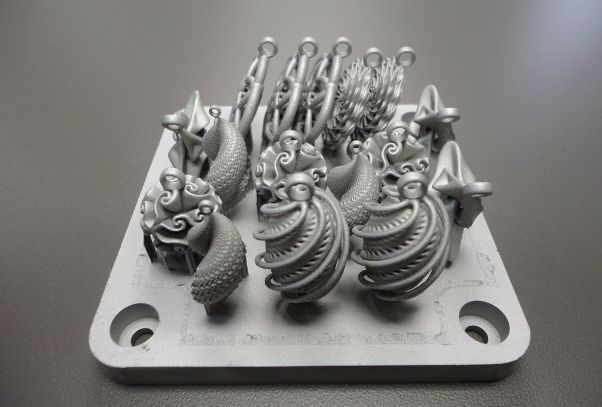
\includegraphics[scale=0.3]{./images/cobalt.png}
\end{figure}\hfill
 \par\leavevmode\par
Grâce au procédé EBM (Electron Beam Melting), une technique voisine du SLS consistant à fusionner une poudre avec un faisceau électron, l'alliage Cobalt Chrome peut désormais être imprimé en 3D. Le suédois Arcam propose par exemple l'ASTM F75, un alliage très solide résistant à l'usure et la corrosion pour concevoir de l'outillage ou des moules. Lisse et résistant, le CoCrMo est un autre alliage employé pour les prothèses de genou ou de hanche par exemple ou des couronnes dentaires. Toujours dans ce domaine EOS a développé Le Chrome Cobalt EOS SP2 un super-alliage pulvérulent destiné aux restaurations dentaires.\hfill
 \par\leavevmode\par
\fbox{
\begin{minipage}{1\textwidth}
Environ 250\euro{} le kg
\end{minipage}}

\subsubsection{Les matériaux précieux}
\begin{figure}[h!]
\centering
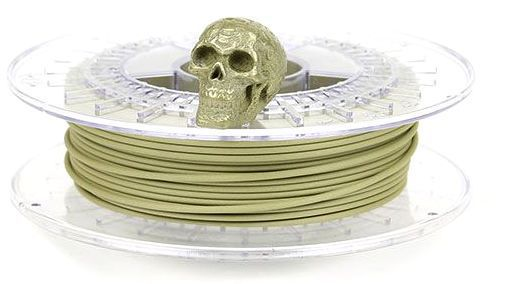
\includegraphics[scale=0.3]{./images/brassfill.png}
\end{figure}\hfill
 \par\leavevmode\par
Les matériaux précieux tels que l'or, l'argent, le platine ou le cuivre ne peuvent pas être directement imprimés en 3D, mais coulés dans des moules conçus par impression 3D. Pour la création de bijoux, on applique une technique de moulage appelée le moulage à la cire perdue. Concrètement vous moulez votre objet en cire afin de créer un moule en plâtre dans lequel est ensuite coulé le métal fondu.\hfill
 \par\leavevmode\par
Pour autant s'il n'est pas possible d'imprimer des métaux précieux à l'état pur, des filaments composites imitant leur apparence ont fait leur apparition sur le marché. Un fabricant Hollandais du nom de ColorFabb s'en est d'ailleurs fait une spécialité. Celui-ci a développé tout une série de filaments composites métalliques à base de PLA et de certains métaux précieux : BrassFill imitant l'or, CopperFill à base de cuivre et Bronzefill à base de bronze.\hfill
 \par\leavevmode\par
\fbox{
\begin{minipage}{1\textwidth}
En moyenne 50\euro{}la bobine de 750g
\end{minipage}}
\newpage
\subsubsection{La céramique}
\begin{figure}[h!]
\centering
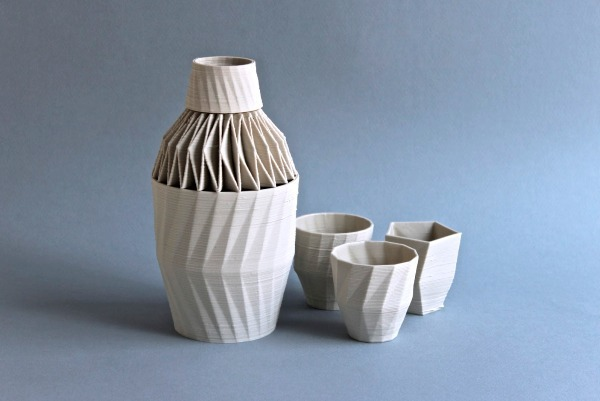
\includegraphics[scale=0.3]{./images/ceramique.png}
\end{figure}\hfill
 \par\leavevmode\par
Normalement, l'impression en céramique fait appel à un procédé spécifique appelé le frittage laser, l'objet subit ensuite un traitement par émaillage à plus de 1000\degres C. Il permet de reproduire un objet qui pourra être réutilisé fonctionnellement dans son environnement réel. En plus d'être alimentaire, le matériau est étanche et recyclable. Idéal pour la fabrication de tasses, soucoupes, assiettes et même de figurines.\hfill
 \par\leavevmode\par
À Andenne, ville de la céramique, nous avons des imprimantes 3d céramique (en prototype) fonctionnelles. Ces dernières utilisent la technologie classique de l'impression 3D.
\newpage

\subsection{Les imprimantes}
\paragraph{Combien coùte une imprimante 3D ?} \hfill 
 \par\leavevmode\par
La question du prix est certainement celle qui revient le plus souvent chez tous ceux, et toutes celles  qui découvrent l'impression 3D. Il existe aujourd'hui sur le marché, une très large gamme de machines, pour toutes sortes d'applications et à tous les tarifs. De quelques centaines d'euros pour une imprimante 3D de bureau à plusieurs centaines de milliers d'euros pour une machine industrielle, l'éventail de modèles est aujourd'hui extrêmement vaste.\hfill
 \par\leavevmode\par
Avec l'expiration successive de nombreux brevets le prix moyen des imprimantes 3D personnelles a été divisé par 10 en 10 ans à peine. Étant donné le marché actuel et la multiplicité des imprimantes 3D voyant le jour, nous allons nous concentrer ici sur les principaux modèles.\hfill
 \par\leavevmode\par
Les imprimantes 3D personnelles peuvent être divisées dans 2 grandes familles :
\begin{itemize}
\item Celles qui sont livrées entièrement montées et prêtes à l'emploi
\item Celles qui sont en kit (de 300\euro{} à 1200\euro{})
\end{itemize}\hfill
 \par\leavevmode\par
Voici quelques prix pour des imprimantes prêtes à l'emploi

\subsubsection{Les Makerbot : 1700 à 7800\euro{}}
\begin{figure}[h!]
\centering
\includegraphics[scale=0.4]{./images/makerbot.png}
\caption{Bre Pettis, fondateur de Makerbot}
\end{figure}\hfill \break
Fondée en 2009 à New York, Makerbot est la première entreprise à avoir commercialisé des imprimantes 3D grand public. Leader incontesté sur ce marché, ce fabricant américain aurait déjà vendu près 100 000 imprimantes depuis 2009.
\newpage
\paragraph{Replicator 2 : 2200\euro{}} \hfill
\begin{figure}[h!]
\centering
\includegraphics[scale=0.4]{./images/replicator2.png}
\end{figure}\hfill \break
Sorti en 2012, la Replicator 2 reste le modèle le plus connu et le plus emblématique de la marque. Si celle-ci n'imprime que sur filament PLA, elle dispose néanmoins d'une bonne résolution (100 microns) et d'un volume de fabrication (28x15x15 cm ) supérieur à la moyenne.

\paragraph{Replicator 2x : 3000\euro{}} \hfill
\begin{figure}[h!]
\centering
\includegraphics[scale=0.4]{./images/replicator2X.png}
\end{figure}\hfill \break
La 2x est une autre version sortie un an plus tard, une variante équipée d'un double extrudeur lui permettant d'imprimer en bicolore ou deux matériaux différents et d'un caisson pour protéger le consommable.
\newpage
\paragraph{Replicator Mini : 1700\euro{}} \hfill
\begin{figure}[h!]
\centering
\includegraphics[scale=0.4]{./images/replicator-mini2.png}
\end{figure}\hfill \break
Par définition la mini possède un volume de fabrication (10x10x12,5) moins élevé que ses grandes sœurs. D'une résolution haute de 200 microns, celle-ci comprend néanmoins plusieurs innovations, une tête d'impression intelligente permettant de détecter le niveau restant de matière ou encore d'une caméra pour surveiller et contrôler vos impressions à distance et un écran tactile.

\paragraph{Replicator 5ème génération : 3500\euro{}} \hfill
\begin{figure}[h!]
\centering
\includegraphics[scale=0.4]{./images/replicator-5G.png}
\end{figure}\hfill \break
Plus grande que la mini, celle-ci se destine à des utilisateurs plus aguerris. On y retrouve les mêmes
innovations techniques que la mini mais avec une meilleure finition allant jusqu'à 100 microns et un volume d'impression plus important : 25x19x15 cm.
\newpage
\paragraph{Replicator Z18 : 7800\euro{}} \hfill
\begin{figure}[h!]
\centering
\includegraphics[scale=0.4]{./images/replicator-z18.png}
\end{figure}\hfill \break
La Z18 qui s'adresse à une clientèle professionnelle est la plus grande de la gamme. Elle dispose de ce fait d'un volume de fabrication particulièrement élevé (30 x 30 x 45 cm) mais aussi d'une chambre d'impression hermétique.

\subsubsection{3D Systems : 600 à 3800\euro{}}
\begin{figure}[h!]
\centering
\includegraphics[scale=0.4]{./images/3d-systems.png}
\caption{Bre Pettis, fondateur de Makerbot}
\end{figure}\hfill \break
Fondé en 1986 en Californie, 3D Systems est à l'origine même de l'impression 3D. En effet son fondateur, un ingénieur du nom de Chuk Hull a breveté en 1984 un procédé appelé SLA (Stéréolithographie), une technique d'impression par rayon UV. 4 ans plus tard la première imprimante 3D SLA voyait le jour... Ce pionnier de l'imprimante 3D et concurrent direct de Stratasys est un poids lourd du marché présent sur de nombreux procédés grâce à ses 1300 brevets. 
\newpage
\paragraph{La Cube 3 : 600\euro{}} \hfill \break
\begin{figure}[h!]
\centering
\includegraphics[scale=0.4]{./images/cube-3.png}
\end{figure}\hfill \break
Il s'agit du modèle nouvelle génération de 3D Systems, une version améliorée de la Cube X avec un design beaucoup plus moderne et soigné. Si son volume d'impression est moindre (152,5 x 152,5 x 152,5 mm), sa résolution a été revue à la hausse (70 microns). De plus celle-ci est dotée d'une double tête d'extrusion pour combiner les matériaux et les couleurs.

\paragraph{La Cube 2 : 845\euro{}} \hfill \break
\begin{figure}[h!]
\centering
\includegraphics[scale=0.4]{./images/imprimante-3d-cube.png}
\end{figure}\hfill \break
Très compacte (4kg), la Cube 2 incarne parfaitement l'imprimante 3D de bureau. Dotée d'un plateau chauffant, la machine est compatible aussi bien avec l'ABS que le PLA, matériaux déclinés dans 16 couleurs différentes. L'appareil dispose d'un volume d'impression de 14x14x14 cm pour une épaisseur de couche de 250 microns.
\newpage
\paragraph{Cube X Mono : 2400\euro{}/ Cube X Duo : 2800\euro{} / Cube X Trio : 3800\euro{}} \hfill \break
\begin{figure}[h!]
\centering
\includegraphics[scale=0.4]{./images/cubex1.png}
\end{figure}\hfill \break
Certifiée pour un usage domestique et destinée aussi bien aux adultes qu'aux enfants, la Cube X est le haut de gamme de 3D Systems. Déclinée en 3 versions avec selon 1,2 ou 3 extrudeurs, il s'agit d'une imprimante personnelle mais avec les qualités techniques d'une semi professionnelle. Avec son volume de fabrication (27,5 x 26,5 x 24 cm) et sa résolution de 125 microns, elle rivalise avec les Replicator 2.

\paragraph{La Cube Pro : 2500\euro{}} \hfill \break
\begin{figure}[h!]
\centering
\includegraphics[scale=0.4]{./images/cubepro.png}
\end{figure}\hfill \break
Toute aussi soignée que la Cube 3D elle s'adresse à une clientèle un peu plus exigeante. Si sa résolution d'impression est similaire (70 microns), son volume d'impression est bien plus élevé: 27,5 x 26,5 x 24 cm. De plus la Cube Pro peut s'équiper de 3 extrudeurs permettant ainsi d'imprimer dans trois couleurs et matériaux différents. Outre l'ABS et le PLA elle peut aussi imprimer avec du nylon.
\newpage
\subsubsection{Les autres marques}
\paragraph{Da Vinci : 600\euro{}} \hfill \break
\begin{figure}[h!]
\centering
\includegraphics[scale=0.1]{./images/davinci.png}
\end{figure}\hfill \break
Ce modèle développé par le taïwanais Kinpo et vendu sous la marque XYZprinting, est sûrement l'un des meilleurs qualité prix du moment. Proposée à 600\euro{}, la Da Vinci offre un volume d'impression de 20 x 20 x 20 cm pour une résolution de 100 microns. Elle fonctionne avec ses propres cartouches d'ABS et de PLA vendue pour 50\euro{} environ les 600g et déclinées dans 13 couleurs.

\paragraph{Ultimaker 2 : 1459\euro{}} \hfill \break
\begin{figure}[h!]
\centering
\includegraphics[scale=0.4]{./images/ultimaker-2.png}
\end{figure}\hfill \break
Issue du fabricant néerlandais Ultimaker, l'Ultimaker 2 propose un volume de fabrication légèrement supérieur au modèle original (230 x 225 x 205 mm), avec design plus soigné grâce notamment à son châssis aluminium. Ce modèle est équipé d'un écran LCD pour faciliter les paramétrages et d'un lecteur SD qui permet à l'imprimante d'être autonome sans avoir à être raccordée à un ordinateur pour transférer vos fichiers 3D. Compatible avec un large panel de filament (3mm), l'Ultimaker 2 reste l'un des modèles les plus rapides du marché (300mm/s) et les plus précis (jusqu'à 20 microns).
\newpage
\paragraph{Zortrax M200 : 1990\euro{}} \hfill \break
\begin{figure}[h!]
\centering
\includegraphics[scale=0.4]{./images/zortrax-M200.png}
\end{figure}\hfill \break
La M200 que l'on doit au constructeur polonais Zortrax a été la bonne surprise de l'année 2014. Cette imprimante 3D de bureau sortie de nulle part, est vite rentrée dans la cour des grands. Très prisée par les makers et de plusieurs fois récompensée (Make, 3D Hubs...), la Zortrax M200 a acquis une notoriété fulgurante en l'espace de quelques mois. Dotée d'un design à la fois sobre et esthétique, cette machine propose un volume d'impression de 20 x 20 x 18,5 cm pour une épaisseur de couches pouvant descendre jusqu'à 25 microns. Fonctionnant sur bobine propriétaire, la M200 est particulièrement efficace lorsqu'il s'agit d'imprimer des matériaux résistants pour la fabrication de produits finis ou de prototypes fonctionnels.
\paragraph{EX1 Basic : 699\euro{}} \hfill \break
\begin{figure}[h!]
\centering
\includegraphics[scale=0.4]{./images/3d-freesculpt.png}
\end{figure}\hfill \break
La EX1 Basic de 3D FreeSculpt fait partie des modèles les moins chers du marché. Possédant une capacité d'impression de 22,5 x 14,5 x 15 cm celle-ci est dotée d'un écran LCD pour contrôler certains paramètres comme la température et la durée d'impression. L'imprimante se décline en plusieurs bundles, 2 packs sont ainsi proposés : La EX1-Plus qui comprend le modèle de base + un logiciel 3D pour 899,90\euro{} et la EX1-ScanCopy, le package complet qui inclus en supplément un scanner 3D pour 1099,90\euro{}
\paragraph{Leapfrog Creatr HS : 2390\euro{}} \hfill \break
\begin{figure}[h!]
\centering
\includegraphics[scale=0.4]{./images/Creatr.png}
\end{figure}\hfill \break
La HS qui signifie High Speed (haute vitesse) est comme son nom l'indique une version améliorée de
la Creatr Originale, avec une vitesse d'impression parmi les plus élevée soit 300mm/s. Elle représente
dans sa gamme un des plus plus gros volumes de fabrication (29 x 24 x 18 cm) et une des meilleures
résolutions (jusqu'à 50 microns). Simple et élégante, cette imprimante comporte une double tête
d'extrusion permettant d'imprimer dans deux couleurs ou deux matériaux différents.
\paragraph{Witbox : 1700\euro{}} \hfill \break
\begin{figure}[h!]
\centering
\includegraphics[scale=0.4]{./images/witbox.png}
\end{figure}\hfill \break
La Witbox de Bq est l'imprimante personnelle proposant l'un des plus gros volumes d'impression du marché : 29,7x21x20 cm. Elle peut de ce fait imprimer des pièces de grandes tailles et en bicolore grâce à son double extrudeur. La Witbox n'imprime que dans le PLA.
\newpage
\paragraph{Up Plus 2 : 1390\euro{}} \hfill \break
\begin{figure}[h!]
\centering
\includegraphics[scale=0.4]{./images/up-plus-2.png}
\end{figure}\hfill \break
Elue en 2014 comme l'imprimante 3D la plus fiable par le magazine Make, la Up Plus 2 a toutes qualités nécessaires pour imprimer maquettes et prototypes. Avec une résolution de 150 microns, ce modèle de la marque PP3DP est un outil efficace et peu encombrant.
\paragraph{Up Mini : 795\euro{}} \hfill \break
\begin{figure}[h!]
\centering
\includegraphics[scale=0.4]{./images/up-mini.png}
\end{figure}\hfill \break
Dernier modèle de PP3DP, la UP Mini est une imprimante fermée, compacte et facile d'utilisation. Idéale pour commencer celle-ci est équipée d'un plateau chauffant, lui permettant ainsi d'imprimer l'ABS, le PLA et le PVA. D'une résolution haute de 200 microns, son volume d'impression est de 12 x 12 x 12 cm.
\newpage
\paragraph{Beethefirst : 1700\euro{}} \hfill \break
\begin{figure}[h!]
\centering
\includegraphics[scale=0.4]{./images/Beethefirst.jpg}
\end{figure}\hfill \break
De la marque portugaise Beeverycreative, Beethefirst se distingue par son design original et son format parfaitement adapté à une utilisation domestique. Grâce à sa poignée vous pourrez la transporter très facilement. Imprime sur un PLA propriétaire.
\paragraph{Dagoma Discoeasy 200} \hfill \break
\begin{figure}[h!]
\centering
\includegraphics[scale=0.4]{./images/dagoma.png}
\end{figure}\hfill \break
Issue de jeunes entrepreneurs français, DAGOMA vous propose une imprimante en kit à 299\euro{} ou 399\euro{} montée. Très bon rapport qualité prix. La société a même une implantation à Roubaix. Pour la Belgique, c'est un plus, car on peut facilement les contacter ou avoir un rendez-vous avec eux.
\newpage
\section{En quoi consiste la modélisations 3D ?}
\subsection{Comment créer un fichier 3D ?}
En dehors du fonctionnement même d'une imprimante 3D et des différentes techniques d'impression 3D existantes, il est important de bien comprendre les différentes étapes de préparation qui précèdent la phase de fabrication. En effet, l'impression 3D commence par un fichier numérique appelé fichier 3D sans lequel il n'est pas possible d'imprimer un objet.
 \par\leavevmode\par
Le fichier 3D qui correspond au modèle virtuel de la pièce, et le logiciel, l'outil qui permet de le dessiner en trois dimensions, sont des éléments essentiels à la conversion d'une image 2D en un objet 3D. Pour créer un modèle 3D il existe plusieurs méthodes. La première consiste à modéliser l'objet que l'on souhaite imprimer en 3D.
 \par\leavevmode\par
\begin{figure}[h!]
\centering
\includegraphics[scale=0.4]{./images/modelisation-3D.png}
\end{figure}\hfill
\subsubsection{La modélisation 3D}
Pour imprimer un objet, sauf rares exceptions, avoir un fichier 3D est une obligation. Celui-ci peut être créé à partir d'un logiciel de modélisation 3D, récupéré directement sur un site spécialisé ou via un scan 3D. Pour concevoir une pièce en 3D, la première solution consiste à la modéliser c'est-à-dire la dessiner en trois dimensions. Pour ce faire, il existe un large éventail de logiciels à votre disposition que l'on peut répartir dans trois grands groupes :
\paragraph{Les modeleurs volumiques}\hfill\break
Ces modeleurs permettent de travailler des objets aux formes simples et primitives : cylindriques, cubiques, rectangulaires, sphériques... A l'instar d'un sculpteur, on conçoit la pièce par ajout, soustraction ou assemblage de formes. Ils sont très utilisés pour la fabrication de pièces mécaniques.

Parmi les plus connus on pense à Solid Edge, CATIA, Autodesk (Tinkercad) et bien sûr Solidworks .
\paragraph{Les modeleurs surfaciques}\hfill\break
Les modeleurs surfaciques qui définissent mathématiquement la surface de l'objet sont généralement très employés dans le domaine artistique pour le design, pour la sculpture digitale et les formes organiques. On peut citer par eux les logiciels Rhinocéros et Catia de Dassault Systèmes.
\paragraph{Les modeleurs paramétriques}\hfill\break
Ces modeleurs s'adressent avant tout aux professionnels tels que les ingénieurs ou les architectes. Avec lui, on modélise non pas en dessinant mais en programmant grâce des équations que l'on peut paramétrer à sa guise. Il permet de créer aussi bien des pièces mécaniques que des objets aux formes organiques (engrenages, bijoux...). OpenSCAD et Rhinocéros (via la fonctionnalité Python) font parti des plus connus.

Quelque soit le modeleur, outre le fait de pouvoir travailler des formes géométriques complexes, il permet également de jouer sur les couleurs, les textures, la luminosité... Le choix du modeleur sera fonction de la nature de l'objet, de ses applications (sculpture, pièce mécanique, architecturale...) mais aussi du budget et des compétences de l'utilisateur dans ce domaine.
\subsubsection{Le scan 3D}
\begin{figure}[h!]
\centering
\includegraphics[scale=0.4]{./images/scanner-dimbody.png}
\end{figure}\hfill \break
Une méthode consiste à numériser l'objet que l'on souhaite imprimer avec un scanner 3D. Parmi les nombreux modèles sur le marché, on distingue plusieurs familles :
\begin{itemize}
\item Les scanners dits à lumière structurée émettent différent type de rayonnement : rayon x, laser, lumière... qui sont projetés sur l'objet pendant qu'une caméra procède à l'analyse de la déformation de la projection.
\item Les scanners laser fonctionnent un peu de la même manière que les télémètres laser qui sert à mesurer les distances. Des milliers de points laser sont projetés sur l'objet cible ce qui donne des milliers de points sur la surface de celui, chacun correspondant à une coordonnée spatiale. Parmi les plus connus ont peut citer le modèle Faro ou encore NextEngine.
\item Les scanners stéréoscopiques fonctionnent avec deux systèmes de caméras vidéo pointant toutes les deux vers le même objet. Le principe est le même que ce que l'on appelle la vision stéréoscopique humaine . Quand nous regardons quelque chose, notre œil droit et notre œilgauche envoie chacun sa propre information au cerveau qui va reconstituer l'image à partir des deux images reçues. 
\item La kinect, il s'agit là de la méthode la moins chère du marché même si elle n'est pas la plus précise. Celle-ci est à la base un périphérique de la console de jeu Xbox, il s'agit d'une petite caméra qui détecte les mouvements et les images. Cette technique a été détournée de son usage initial pour jouer le rôle d'un scanner en la couplant à différents logiciels tels que Scenect, Skanet ou encore ReconstructMe.
\end{itemize}
\subsubsection{Récupérer ses fichiers 3D sur des plateformes}
La méthode la plus simple si vous n'avez ni les moyens ni la compétence technique, c'est de récupérer directement votre fichier sur une plateforme de partage.


Il existe une multitude de sites web proposant gratuitement ou pas ce genre de modèles. On peut déjà citer parmi les sites français, Sketchfab une plateforme gratuite créée en 2012 qui dispose déjà de 100 000 modèles en ligne. Sa particularité c'est le pouvoir de pouvoir y échanger et visualiser les plans 3D directement via le navigateur.

Il y a aussi l'inévitable Sculpteo mais qui est un cas particulier, car il s'agit d'un service d'impression 3D. De ce fait pour ce site il n'est pas possible de télécharger des fichiers pour votre imprimante, vous choisissez votre modèle 3D que Sculpteo va ensuite imprimer pour vous. 

Du côté des sites étrangers le choix est bien plus vaste... On retrouve bien sûr Thingiverse , la boutique en ligne de l'américain Makerbot. Parmi les plus connus, on ne peut oublier 3D Warehouse la fameuse banque d'images de sketchup google, mais aussi Shapeway qui est certainement la plus connue et que l'on pourrait même qualifier d'amazon de l'impression 3D. Pour cette plateforme néerlandaise, à l'instar de Sculpteo, pas de téléchargement possible mais on peut y trouver des modèles à faire imprimer ou même y vendre ses propres créations.
\newpage
\subsubsection{Le format STL}
\begin{figure}[h!]
\centering
\includegraphics[scale=0.4]{./images/fichier-stl.png}
\end{figure}\hfill 

Quelque soit la méthode que vous avez choisi ci-dessus pour récupérer un fichier, celui-ci devra être exporté au format STL pour que l'impression puisse se lancer. Inventé par 3D Systems, ce format ne sert qu'à transmettre la géométrie de surface de votre objet. Le fichier qui est exporté se présente sous la forme d'un maillage composé de plusieurs triangles déterminant le volume de votre objet dans l'espace. Il faut veiller à ce que ce maillage soit bien fermé pour que celui-ci soit considéré comme solide, de plus sa qualité est importante car jouant sur le résultat final de votre impression. Même si tous les logiciels n'exportent pas au format STL, souvent il suffit de modifier l'extension pour parer au problème.
\paragraph{Préparation du fichier STL}\hfill
 \par\leavevmode\par
Avant de lancer l'impression il reste une dernière opération. Un logiciel va devoir découper en plusieurs tranches ce fichier STL, chacune d'entre elles représentant une portion du modèle à imprimer. Plus la résolution sera mince plus il faudra de tranches et donc plus se sera long. Si vous avez par exemple une résolution de 50 microns (5 tranches/mm) cela correspond à 50 tranches par cm. C'est également à ce moment qu'est calculée la densité de votre pièce, c'est-à-dire la quantité de matière qu'il va être nécessaire pour la remplir ainsi que l'épaisseur de sa surface externe. Entre par exemple un vase et un engrenage, la densité n'est pas la même...
 \par\leavevmode\par
En règle général chaque imprimante 3D a déjà son propre logiciel de tranchage intégré, parmi les plus courants on retrouve Cura, Markerware, KiSSlicer, Slic3r, ReplicatorG... Le fichier tranché se fera exclusivement dans le format G-code qui est un langage de commande presque universel pour les machines outils.
\newpage
\subsubsection{Un support pour votre projet}
\begin{figure}[h!]
\centering
\includegraphics[scale=0.4]{./images/raftmakerbot.png}
\end{figure}\hfill

Si vous pratiquez une impression de type FDM, l'ajout d'une grille de fabrication appelée raft (en dessous de la pièce) ou brim (autour de la pièce), est parfois recommandée afin de soutenir votre objet. Ce support permet d'éviter que votre pièce ne se décolle du plateau (phénomène appelé warping), surtout si sa base est réduite. Le dépôt couche par couche se fera sur cette base pour empêcher la pièce de s'effondrer. Ce genre de support est le plus souvent utilisé pour les filaments de type ABS ou nylon dont les bords ont tendance à se décoller du fait de la rétractation du plastique lorsque celui-ci refroidi, surtout si l'imprimante 3D ne dispose pas de plateau chauffant.
\begin{figure}[h!]
\centering
\includegraphics[scale=0.4]{./images/raft-cerf.png}
\end{figure}\hfill

Pour d'autres objets tels que par exemple des figurines ou une fusée, une structure de soutien (sorte d'échafaudage) sera nécessaire pour soutenir la pièce durant l'impression. C'est le logiciel de tranchage qui détermine l'emplacement de ces supports et la quantité de matière à déposer selon une trame bien précise pour pouvoir l'enlever plus facilement une fois l'impression terminée.
\newpage
\subsubsection{Exportation du fichier}
Il y a plusieurs façons d'exporter un fichier 3D. Tout dépend en fait du type d'imprimante 3D utilisée. Selon les marques et les modèles, l'exportation s'effectue via un câble USB, d'autres via wifi ou encore avec une carte SD. Pour la majorité des imprimantes 3D qui sortent aujourd'hui sur le marché, le transfert du fichier 3D peut se faire via toutes ces options, avec en plus le Wi-Fi.
\subsection{Droits d'auteur ? Licences ?}
\fbox{
\begin{minipage}{1\textwidth}
\textbf{ATTENTION} 

Il est de bon ton de distinguer les cas de contenus libres de droit des cas de contenus protégés par le droit des propriétés intellectuelles. Contrairement à ce que cela pourrait laisser supposer, libre de droit ne signifie pas absence de droit.
\end{minipage}}
\paragraph{Bouleversement juridique}\hfill

Les questionnements juridiques liés à l'impression 3D concernent surtout les dessins et modèles protégés par le droit de la propriété intellectuelle. Force est de constater qu'aucune législation spécifique n'encadre le droit des créations d'objets par impression 3D. C'est pourquoi le droit intellectuel “classique” trouve en général à s'appliquer.
 \par\leavevmode\par
En d'autres termes, cela signifie que, pour que soit contestée la vente d'objets issus de l'impression 3D et représentants un contenu susceptible d'être couvert par le droit d'auteur, il faut attendre que les ayants droit (détenteur du droit d'auteur) se manifestent.
 \par\leavevmode\par
On peut alors légitimement se demander en quoi les dispositions relatives aux dessins et modèles seraient à même de concerner l'impression d'objet 3D.
 \par\leavevmode\par
Voici quelques articles du Code de la propriété intellectuelle valable également en Belgique : 
\begin{itemize}
\item \textbf{article L. 511-1} : « peut être protégée à titre de dessin ou modèle l'apparence d'un produit, ou d'une partie de produit, caractérisée en particulier par ses lignes, ses contours, ses couleurs, sa forme, sa texture ou ses matériaux. »
\item \textbf{article L.511-2} : « est regardé comme un produit tout objet industriel ou artisanal, notamment les pièces conçues pour être assemblées en un produit complexe, les emballages, les présentations, les symboles graphiques et les caractères typographiques, à l'exclusion toutefois des programmes d'ordinateur » . À ce titre, les objets en trois dimensions sont des objets protégés par le droit des dessins et modèles
dès lors qu'ils font l'objet d'un enregistrement (article L. 511-9 Code de la propriété intellectuelle).
\item \textbf{article L. 513-2} : « l'enregistrement d'un dessin ou modèle concède un droit de propriété au demandeur à l'enregistrement portant sur le dessin ou modèle en cause » .
\item \textbf{article L. 513-4} : « sont interdits, à défaut du consentement du propriétaire du dessin ou modèle, la fabrication, l'offre, la mise sur le marché, l'importation, l'exportation, l'utilisation, ou la détention à ces fins, d'un produit incorporant le dessin ou modèle » .
\item \textbf{article 513-6 a} : « la protection conférée par le droit des dessins et modèles ne s'applique pas pour des reproductions faites à titre privé dans un but non-commercial. On peut légitimement considérer l'impression d'objet 3D, enregistré à titre de dessin ou modèle, comme la fabrication d'une copie sans le consentement du propriétaire du dessin ou modèle. Si ces objets sont par la suite commercialisés, l'atteinte est dès lors qualifiée » .
\item \textbf{article L. 521-1} : « les actes définis à l'article L. 513-4 constituent une contrefaçon engageant la responsabilité civile de son auteur » .
\end{itemize}
 \par\leavevmode\par
On peut donc logiquement conclure que même en l'absence de dispositions propres à l'impression 3D
d'objets protégés par le droit des marques et dessins, le code de la propriété intellectuelle est voué à
s'appliquer et que la fabrication de ces objets, en vue d'une commercialisation, constitue une atteinte
au droit de propriété du titulaire de l'enregistrement qui peut dès lors engager une action en
contrefaçon de dessin ou modèle.
 \par\leavevmode\par
\paragraph{Rappel : Licences Creative Commons}
 \par\leavevmode\par
\begin{figure}[h!]
\centering
\includegraphics[scale=0.42]{./images/licences.png}
\end{figure}\hfill 

\section{Modélisation 3D}
\subsection{Rappels}
\paragraph{Comment ça marche ?}
 \par\leavevmode\par
\begin{figure}[h!]
\centering
\includegraphics[scale=0.35]{./images/infographie.png}
\end{figure}\hfill
\paragraph{1D - 2D - 3D}
 \par\leavevmode\par
\begin{figure}[h!]
\centering
\includegraphics[scale=0.3]{./images/2-3d.png}
\end{figure}\hfill 
\newpage
\subsection{Pour les graphistes}
\begin{figure}[h!]
\centering
\includegraphics[scale=0.35]{./images/blender.png}
\end{figure}\hfill 
Blender - Logiciel libre et gratuit (à installer)
https://www.blender.org/
 \par\leavevmode\par
\begin{figure}[h!]
\centering
\includegraphics[scale=0.3]{./images/freecad.png}
\end{figure}\hfill 
FreeCAD - Logiciel libre et gratuit (à installer)
http://freecadweb.org/
\newpage
\begin{figure}[h!]
\centering
\includegraphics[scale=0.3]{./images/sketchup.png}
\end{figure}\hfill
 \par\leavevmode\par
Google Sketchup (à installer)
http://www.sketchup.com/fr
\begin{figure}[h!]
\centering
\includegraphics[scale=0.3]{./images/tinkercad.png}
\end{figure}\hfill
 \par\leavevmode\par
TINKERCAD (online)
http://www.tinkercad.com
\begin{figure}[h!]
\centering
\includegraphics[scale=0.3]{./images/cookiecaster.png}
\end{figure}\hfill 
 \par\leavevmode\par
Cookie Caste (online) - pour les fans de cuisine
https://www.cookiecaster.com/
\newpage
\subsection{Pour les non-graphistes ou les pressés}
Vous ne savez pas dessiner ? Pas d'inquiétude, voici une liste de sites où vous trouverez des modèles prêts à être imprimés.
\begin{figure}[h!]
\centering
\includegraphics[scale=0.3]{./images/thingiverse.png}
\end{figure}\hfill 
 \par\leavevmode\par
Thingiverse
http://www.thingiverse.com/
\begin{figure}[h!]
\centering
\includegraphics[scale=0.3]{./images/youmagine.png}
\end{figure}\hfill 
 \par\leavevmode\par
Youmagine
https://www.youmagine.com/
\newpage
\begin{figure}[h!]
\centering
\includegraphics[scale=0.3]{./images/3dwarehouse.png}
\end{figure}\hfill 
 \par\leavevmode\par
3D Warehouse - Moteur de Google Sketchup
https://3dwarehouse.sketchup.com/
\begin{figure}[h!]
\centering
\includegraphics[scale=0.3]{./images/cults.png}
\end{figure}\hfill 
 \par\leavevmode\par
Cults 3D
https://cults3d.com/fr
\begin{figure}[h!]
\centering
\includegraphics[scale=0.3]{./images/yeggi.png}
\end{figure}\hfill 
 \par\leavevmode\par
yeggi - Moteur de recherche
http://www.yeggi.com/

\part{Pratique}
\setcounter{section}{0}
\section{Canal d'impression type}
\begin{figure}[h!]
\centering
\includegraphics[scale=0.35]{./images/canalimpression.png}
\end{figure}\hfill
\newpage
\section{Logiciel d'impression (Slicer)}
Pour les besoins du cours, nous allons utiliser un logiciel libre et gratuit : Cura d'Ultimaker qui fonctionne avec plusieurs imprimantes de différentes marques.
\begin{figure}[h!]
\centering
\includegraphics[scale=0.25]{./images/cura1.png}
\end{figure}\hfill 

\begin{figure}[h!]
\centering
\includegraphics[scale=0.25]{./images/cura2.png}
\end{figure}\hfill 
\newpage
\begin{figure}[h!]
\centering
\includegraphics[scale=0.6]{./images/cura3.png}
\end{figure}\hfill 

\begin{figure}[h!]
\centering
\includegraphics[scale=0.25]{./images/cura5.png}
\end{figure}\hfill 

\begin{figure}[h!]
\centering
\includegraphics[scale=0.6]{./images/cura6.png}
\end{figure}\hfill 
\newpage
\begin{figure}[h!]
\centering
\includegraphics[scale=0.3]{./images/cura7.png}
\end{figure}\hfill 

\begin{figure}[h!]
\centering
\includegraphics[scale=0.25]{./images/cura9.png}
\end{figure}\hfill 
\newpage
\begin{figure}[h!]
\centering
\includegraphics[scale=0.3]{./images/cura8.png}
\end{figure}\hfill 

\section{Apprentissage de Tinkercad}

\includepdf[pages=1-19]{./pdf/tinkercad.pdf}

\section{Conclusion}
Quelques citations :

\begin{quotation}
La créativité est contagieuse, faites la tourner
\end{quotation}
\begin{flushright}
Albert Einstein
\end{flushright} 

\begin{quotation}
Chaque enfant est un artiste. Le problème, c'est de rester un artiste lorsqu'on grandit
\end{quotation}
\begin{flushright}
Pablo Picasso
\end{flushright} 

\begin{quotation}
La créativité est une drogue dont je ne peux pas me passer
\end{quotation}
\begin{flushright}
Cecil B.DeMille
\end{flushright} 

\begin{center}
{\LARGE À vous de jouer, de créer, de tester ...} 
\end{center}

\section{informations}
\begin{center}
www.denis-sylvain.be

www.yourlab.be

denis-sylvain@perso.be

sylvain@yourlab.be
\end{center}
\end{document}
